\documentclass[11pt,openany]{article}
\usepackage{geometry}
\geometry{
	letterpaper,
	margin=1in
}
\usepackage{blindtext}
\usepackage{tikz,tcolorbox,tikz-3dplot}
\usepackage{pgfplots}
\usepgfplotslibrary{fillbetween}
\usepackage{xcolor}
\usepackage{amsfonts}
\usepackage{hyperref} 
\usepackage{indentfirst}
\usepackage{graphicx}
\usepackage{caption}
\usepackage{subcaption}
\usepackage[normalem]{ulem}
\usepackage [english]{babel}
\usepackage [autostyle, english = american]{csquotes}
\usepackage{appendix}

\usepackage[ruled,linesnumbered]{algorithm2e}
\SetKwComment{Comment}{/* }{ */}
\DontPrintSemicolon 
\usepackage{tabularx}
\usepackage{amsmath,amssymb}
\usepackage{mathtools}
\usepackage{makecell}
\graphicspath{ {./images/} }
\usepackage{enumitem}
\usepackage{soul}
\usepackage{mathtools}
\usepackage{wrapfig}
\usepackage{mathrsfs}
\usepackage{centernot}
\usepackage{amsthm}
\usepackage{listings}
%\usepackage{biblatex}
%\addbibresource{bibliograph.bib}
\usepackage{microtype}
\usepackage{pagenote}
\usepackage{array}
\usepackage{xparse}

\tcbuselibrary{theorems}

\definecolor{codegreen}{rgb}{0,0.6,0}
\definecolor{codegray}{rgb}{0.5,0.5,0.5}
\definecolor{codepurple}{rgb}{0.58,0,0.82}
\definecolor{backcolour}{rgb}{0.95,0.95,0.92}

\lstdefinestyle{mystyle}{
	backgroundcolor=\color{backcolour},   
	commentstyle=\color{codegreen},
	keywordstyle=\color{magenta},
	numberstyle=\tiny\color{codegray},
	stringstyle=\color{codepurple},
	basicstyle=\ttfamily\footnotesize,
	breakatwhitespace=false,         
	breaklines=true,                 
	captionpos=b,                    
	keepspaces=true,                 
	numbers=left,                    
	numbersep=5pt,                  
	showspaces=false,                
	showstringspaces=false,
	showtabs=false,                  
	tabsize=2
}

\lstset{style=mystyle}
%% End notes to be printed as sections at the
%% end of each chapter.
\renewcommand*{\notedivision}{\section*{\notesname}}
\renewcommand*{\pagenotesubhead}[1]{}

%\newcommand*{\exercises}{\section*{\exercisename}}
%%%%%%%%%%%%% For customising the endnote markers. Comment these out if you don't want them.
% To prefix each note number with the chapter number
\renewcommand{\thepagenote}{\thechapter-\arabic{pagenote}}

% To have a slightly different formatting for the endnote numbers in the text -- smaller text, sans-serif, square brackets
\renewcommand\notenumintext[1]{\space{\footnotesize\sffamily[FN-#1]}}

% To have a slightly different formatting for the endnote numbers in the notes section. Just the square brackets and sans-serif; normal size.
\renewcommand\notenuminnotes[1]{{\sffamily[FN-#1] }}
% If you want a different name/heading for the end notes
\renewcommand{\notesname}{End Notes}
\newcommand{\exercisename}{Exercises}
\newcounter{thatonetheorem}
\newcounter{exercisecounter} % continuity of exercises in a section
\newenvironment{exerciselist}{
	\begin{enumerate}
		\setcounter{enumi}{\value{exercisecounter}}
	}{
		\setcounter{exercisecounter}{\value{enumi}}
	\end{enumerate}
}
\newenvironment{thatonethmlist}{
	\begin{enumerate}
		\setcounter{enumi}{\value{thatonetheorem}}
	}{
		\setcounter{thatonetheorem}{\value{enumi}}
	\end{enumerate}
}
\newcommand*{\exercises}{\section*{\exercisename}}

\newcommand\todo{\textcolor{red}{\textbf{TODO: }}}
%%%%%%%%%%%%% End customisation
\newcommand{\stackeq}[1]{\stackrel{\mathclap{\normalfont\mbox{\normalfont\tiny {#1}}}}{=}}
\newcommand{\reals}{\mathbb{R}}
\newcommand\defeq{\mathrel{\stackrel{\makebox[0pt]{\mbox{\normalfont\tiny def}}}{=}}}
\makeatletter
\renewcommand*\env@matrix[1][*\c@MaxMatrixCols c]{%
  \hskip -\arraycolsep
  \let\@ifnextchar\new@ifnextchar
  \array{#1}}
\makeatother

\newcounter{thmcounter} % continuity of theorem

\newcommand{\definition}[2]{\addtocounter{thmcounter}{1}
\begin{tcolorbox}[title=Definition {\thesection}.{\arabic{thmcounter}} ({#1}),colframe=black]
		{#2}\end{tcolorbox}


}
\newcommand{\proposition}[1]{
	\addtocounter{thmcounter}{1}
	\begin{tcolorbox}[title=Proposition {\thesection}.{\arabic{thmcounter}},colframe=red!50!blue!20!white,colback=red!35!blue!10!white, coltitle=black]{#1}\end{tcolorbox}

}
\newcommand{\theorem}[2]{
\addtocounter{thmcounter}{1}
\begin{tcolorbox}[title=\color{black}Theorem {\thesection}.{\arabic{thmcounter}} ({#1}),colframe=red!40,colback=red!5!white]{#2}\end{tcolorbox}
	
}
\newcommand{\lemma}[1]{
\addtocounter{thmcounter}{1}
\begin{tcolorbox}[title=\color{black}Lemma {\thesection}.{\arabic{thmcounter}},colframe=blue!40,colback=blue!5!white]{#1}\end{tcolorbox}
	
}
\newcommand{\example}[1]{\addtocounter{thmcounter}{1}\begin{tcolorbox}[title=Example {\thesection}.{\arabic{thmcounter}},colframe=yellow!20!white,colback=yellow!10!white,coltitle=black]{#1}\end{tcolorbox}


}
\newcommand{\corollary}[1]{	\addtocounter{thmcounter}{1}\begin{tcolorbox}[]{Corollary {\thesection}.{\arabic{thmcounter}}: {#1}}\end{tcolorbox}
	

}


%%% Eliseu's fix for theorem numbering

% Definition
\NewTcbTheorem[number within=section, use counter=thmcounter]{adefinition}{Definition}{
	colframe=black, 
	separator sign none, 
	description delimiters parenthesis}{def}
% Proposition
\NewTcbTheorem[number within=section, use counter=thmcounter]{aproposition}{Proposition}{
	colframe=red!50!blue!20!white,colback=red!35!blue!10!white, coltitle=black,
	separator sign none, 
	description delimiters parenthesis}{prop}
% Theorem
\NewTcbTheorem[number within=section, use counter=thmcounter]{atheorem}{Theorem}{
	colframe=red!40,colback=red!5!white, coltitle=black,
	separator sign none, 
	description delimiters parenthesis}{thm}

% Lemma
\NewTcbTheorem[number within=section, use counter=thmcounter]{alemma}{Lemma}{
	colframe=blue!40,colback=blue!5!white, coltitle=black,
	separator sign none, 
	description delimiters parenthesis}{lemma}
% Example
\NewTcbTheorem[number within=section, use counter=thmcounter]{aexample}{Example}{
	colframe=yellow!20!white,colback=yellow!10!white,coltitle=black,
	separator sign none, 
	description delimiters parenthesis}{ex}
% Corollary
\NewTcbTheorem[number within=section, use counter=thmcounter]{acorollary}{Corollary}{
	separator sign none, 
	description delimiters parenthesis,
	coltitle=black,
	attach title to upper={:\ }}{cor}


%%% Eliseu's fix for backwards compatibility with Chi's macros

\let\olddefinition\definition
\let\oldproposition\proposition
\let\oldtheorem\theorem
\let\oldexample\example
\let\oldcorollary\corollary
\let\oldlemma\lemma

\renewcommand{\definition}[3][\relax]{\ifx\relax#1\olddefinition{#2}{#3}\else \begin{adefinition}{#2}{#1} #3 \end{adefinition} \fi}
\renewcommand{\proposition}[2][\relax]{\ifx\relax#1\oldproposition{#2}\else \begin{aproposition}{}{#1} #2 \end{aproposition} \fi}
\renewcommand{\theorem}[3][\relax]{\ifx\relax#1\oldtheorem{#2}{#3}\else \begin{atheorem}{#2}{#1} #3 \end{atheorem} \fi}
\renewcommand{\example}[2][\relax]{\ifx\relax#1\oldexample{#2}\else \begin{aexample}{}{#1} #2 \end{aexample} \fi}
\renewcommand{\corollary}[2][\relax]{\ifx\relax#1\oldcorollary{#2}\else \begin{acorollary}{}{#1} #2 \end{acorollary} \fi}
\renewcommand{\lemma}[2][\relax]{\ifx\relax#1\oldlemma{#2}\else \begin{alemma}{}{#1} #2 \end{alemma} \fi}
\newtheorem*{remark}{Remark}
\newtheorem*{notation}{Notation}
%\newcommand{\exercises}{\section*{\exercisename}}
%% THIS LINE IS MANDATORY
\makepagenote
\newcommand{\sakura}{
\begin{tikzpicture}
    % Define petal colors
    \definecolor{petalpink}{RGB}{255, 182, 193}
    \definecolor{petaldark}{RGB}{255, 105, 180}
    
    % Draw petals with thinner bases
    \foreach \angle in {0, 72, 144, 216, 288} {
        \begin{scope}[rotate=\angle]
            \fill[petalpink] 
            (0,0) -- (0.3,-0.1) 
            .. controls (0.9,0.5) and (0.6,1.5) .. (0,1.3) 
            .. controls (-0.6,1.5) and (-0.9,0.5) .. (-0.3,-0.1) -- cycle;
			\draw[white] (0,0.4) edge (0,1);

        \end{scope}
		
		
    }
    
    % Add a darker pink center
    \fill[petaldark] (0,0) circle (0.25);

    % Add stamen dots around the center
    \foreach \angle in {-36, 36, 108, 180, 252} {
		\begin{scope}[rotate=\angle]
            \fill[petaldark] (0,0.45) circle (0.08);

        \end{scope}
        
    }

\end{tikzpicture}}

\newcommand{\oldsakura}{
\begin{tikzpicture}
    % Define petal colors
    \definecolor{petalpink}{RGB}{255, 182, 193}
    \definecolor{petaldark}{RGB}{255, 105, 180}
    
    % Draw petals with thinner bases
    \foreach \angle in {0, 72, 144, 216, 288} {
        \begin{scope}[rotate=\angle]
            \fill[petalpink] 
            (0,0) -- (0.3,-0.1) 
            .. controls (0.9,0.5) and (0.6,1.5) .. (0,1.3) 
            .. controls (-0.6,1.5) and (-0.9,0.5) .. (-0.3,-0.1) -- cycle;
        \end{scope}
    }
    
    % Add a darker pink center
    \fill[petaldark] (0,0) circle (0.25);

    % Add stamen dots around the center
    \foreach \angle in {0, 60, 120, 180, 240, 300} {
        \fill[petaldark] ([shift=(\angle:0.45)]0,0) circle (0.05);
    }

    % Add white highlights for detail
    \foreach \angle in {30, 90, 150, 210, 270, 330} {
        \fill[white] ([shift=(\angle:0.6)]0,0) circle (0.03);
    }
\end{tikzpicture}}
\newcommand{\sakuraqed}{1}
\newcommand{\oldqed}{\qedsymbol}
\renewcommand{\qedsymbol}{\if\sakuraqed1 {\raisebox{-0.5ex}{\resizebox{2.5ex}{2.5ex}{\sakura}}}\else {\oldqed}\fi}

\newcommand{\newsection}{\setcounter{thmcounter}{0}}
%\ref{def:label}, \ref{prop:label}, \ref{thm:label}, \ref{ex:label}, \ref{cor:label}.
% \setcounter{thmcounter}{0}
% \begin{atheorem}[foor}{bar}{label} or use square brackets before the function, like 
\setcounter{section}{-1}
\usepackage{titling}
\predate{}
\postdate{}
\date{}
\title{EE 495 Game Theory and Networked Systems}
%\author{Chi Li}
\begin{document}
\maketitle
\section{Syllabus}
\newsection
All logistics are on canvas.

Randy Berry: Office L352.

There are no required texts for the class. There are some references (4) that are suggested on Canvas. 
\subsection*{Prereqs}
\begin{enumerate}
    \item No prior knowledge on game theory is required.
    \item Mathematical background is required. Linear algebra, probability, optimization, mathematical maturity.
\end{enumerate}
\subsection*{Grades}
\begin{itemize}
    \item Midterm: in class, $35\%$
    \item Final project: $35\%$
    \item Problemsets: $30\%$
\end{itemize}
\begin{atheorem}{}{}
    Randy is a chill professor.
\end{atheorem}
\section{Lecture 1: Introduction to Game Theory}
\newsection
\definition{Game Theory}{
    Game theory is the study of interactions of \textit{multiple strategic agents}.
}
Features of game theory:\begin{itemize}
    \item More than one decision makers.
    \item Each agent makes decisions to maximize self-interest.
    \item These \textbf{agents} are players of the `game', and can be people, firms, countries (in political science), AI-agents etc.
\end{itemize}

\example{
    The following are examples of `games':\begin{itemize}
        \item 2 people playing chess. Their incentives do not align because each player wants to checkmate the other.
        \item 2 firms competing in a market. They are selling the similar items and are trying to price their items to get a larger market share.
        \item 4 countries competing to maximize GDP.
    \end{itemize}
}

The other component of this course is network systems.
\example{
    The following are examples of network systems:\begin{itemize}
        \item Communication network. 
        \item Electricity network.
        \item Transportation network.
    \end{itemize}
}
We will use these as examples to illustrate the concepts in game theory. However, the same theory can extend into the other games.
We want to model and analyze games. People are complicated to model, and our models are simplifications of reality. We need to understand what assumptions are made for each models to apply analysis. 

\subsection*{Basic Game Model}
\definition[basicgame]{Basic Game Model}{
    A \textbf{strategic form game} $G$ consists of the following elements:\begin{enumerate}
        \item The set of agents/players $R$, usually enumerated $R=\{1,2,3,\ldots, n\}$.
        \item For every $r\in R$, the action set of player $r$ $S_r$. If $\left|\bigsqcup_r S_r\right|<\infty$, we call the game a \textbf{finite game}.
        \item For every $r\in R$, a payoff function $\pi_r:\otimes_{r'} S_{r'}\to \reals$. Each agent $r$ wants to maximize $\pi_r$. 
    \end{enumerate}
}
That means, there is only one round of this game, and everyone makes the same decision all at once.
\begin{remark}
    The action set can also be called the strategic set.
\end{remark}
\begin{notation}
    The ordered set of everyone's actions except $r$ is \[
        \overline{s_{-r}}=(s_1,s_2,\ldots, s_{r-1},s_{r+1},\ldots,s_n).
    \]
    Therefore player $r$ is actually maximizing \[
    \pi_r(s_r,\overline{s_{-r}}).
    \]
    The second part of this function is outside of $r$'s control.
\end{notation}

\example{
    Consider two Internet Service Providers (ISPs)
    \begin{center} 
    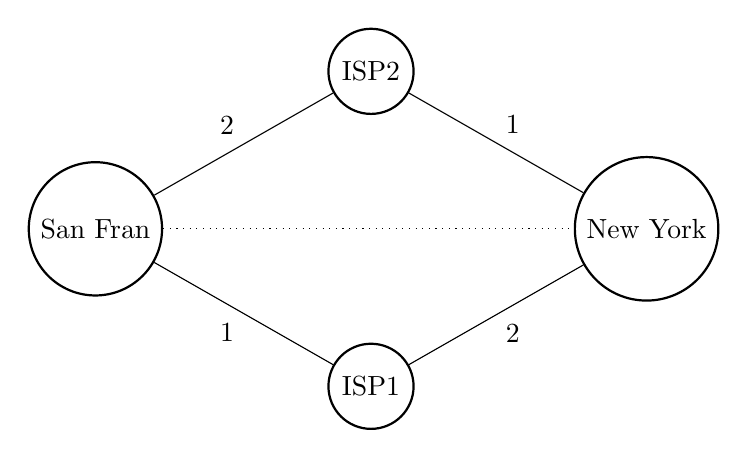
\begin{tikzpicture}
        \begin{scope}[every node/.style={circle,thick,draw}]
        \node (a) at (0,0) {San Fran};
        \node (b) at (7,0){New York};
        \node (c) at (3.5,2){ ISP2};
        \node (d) at (3.5,-2){ ISP1};
        \end{scope}
        \draw [dotted] (a) --  (b);
        \draw (a) -- node[midway, below left]{1}(d) -- node[midway, below right]{2}(b);
        \draw (a)-- node[midway, above left]{2} (c) --node[midway, above right]{1}(b);
    \end{tikzpicture}\end{center}

    They have peered i.e. no charge to send traffic to each other. 
    There is 1MB of traffic to ISP 1 customers in NY. There is 1mB of traffic to ISP 2 in SF. Each ISP will incur the cost of usage of the two (respective) edges connected to it, per mB of traffic.
    Here,\begin{align*}
        R&=\{1,2\}\\
        S_r&=\{\textrm{near},\textrm{far}\}, 
    \end{align*}
    that is, each ISP can decide whether to send the traffic directly or through the other ISP.
}
We can represent this as a matrix 
\iffalse
  ISP1 \ ISP2  near far

near (-4,-4) (-1,-5)

far (-5,-1) (-2,-2)


\fi
\begin{center}
    \begin{tabular}{|c|c c|} 
        \hline
        ISP 1\textbackslash ISP2 & near & far \\ 
        \hline
        near & (-4,-4) & (-1,-5) \\ 
        \hline
        far & (-5,-1) & (-2,-2)\\
        \hline
    \end{tabular}
\end{center}

\definition[dominant]{Dominant action}{
    An Action is $s_r^*$ is \textbf{weakly dominant} if \[
    \pi_r(s_r^*,\overline{s_{-r}})\geq\pi_r(s_r,\overline{s_{-r}})
    \]
    for all $s_r\neq s_r^*$, and any $\overline{s_{-r}}$.
    If inequality is strict, then the action is \textbf{strictly dominant}.
}
\corollary{
    If the game has a strictly dominant action for each player, this will give a unique dominant strategy equilibrium.
}
\example{
    Consider the game with the reward matrix:
    \begin{center}
        \begin{tabular}{|c|c c c|} 
            \hline
            1\textbackslash 2 & L & M & R \\ 
            \hline
            U & (1,0) & (2,-1) & (1,2) \\ 
            \hline
            D & (0,3) & (1,4)& (0,1)\\
            \hline
        \end{tabular}
    \end{center}
    There is no dominant action for player 2, but there is a dominant action (U) for player 1. Therefore, player 2 can rationally assume that player 1 does not play D. Under this assumption, player 2 has a dominant strategy of (R).
}
\example[techorkellog]{
    Alice and Bob want to get lunch together
    Consider the game with the reward matrix:
    \begin{center}
        \begin{tabular}{|c|c c|} 
            \hline
            1\textbackslash 2 & Tech&Kellog \\ 
            \hline
            Tech & (2,3) & (1,1)\\ 
            \hline
            Kellog & (1,1)&(3,2)\\
            \hline
        \end{tabular}
    \end{center}
    There is no dominant action for each player. This is known as a coordination game, it is better to follow what the other player chooses.
}
\definition[nasheq]{Nash Equilibrium}{
    A strategy profile $(s_1^*,\ldots, s_n^*)$ is a \textbf{Nash equilibrium} if \[
    \pi_r(s^*_r,s^*_{-r})\geq\pi_r(s_r,s^*_{-r})
    \]
    for each agent $r$, $s_r\in S_r$.

    In other words, no player benefits from unilateral deviations.
}
In the case of Example \ref{ex:techorkellog}, the two Nash equilibria are when both players pick the same place to eat. However, there are no dominant strategies! Even if we made the matrix 
\begin{center}
    \begin{tabular}{|c|c c|} 
        \hline
        1\textbackslash 2 & Tech&Kellog \\ 
        \hline
        Tech & (5,5) & (1,1)\\ 
        \hline
        Kellog & (1,1)&(2,2)\\
        \hline
    \end{tabular}
\end{center}
there will still be two Nash equilibria, even though the (5,5) outcome is much better than the other (2,2) - some are better than others.

\proposition{
    A dominant strategy equilibrium is a Nash equilibrium.
}
\begin{proof}
    By definition.
\end{proof}
\begin{aexample}{Attacker Defender}{attackdefend}
    
    Consider the reward matrix
    \begin{center}
        \begin{tabular}{|c|c c|} 
            \hline
            Attacker\textbackslash User & A&B \\ 
            \hline
            A & (1,0) & (0,1)\\ 
            \hline
            B & (0,1)&(1,0)\\
            \hline
        \end{tabular}
    \end{center}
    The attacker always wants to choose the channel with the user, but the user wants a different channel. In this case, there is no Nash equilibrium (either the attacker can move to the user channel or the user move away from the attacker channel).
\end{aexample}
\subsection*{Next Time}
Mixed strategies, thm: finite game with randomized strategies always have nash equilibria.
\section{Lecture 2: Games with Continuous Strategies}
\newsection
\subsection*{Recap of last lecture}
\begin{enumerate}
    \item Definition of Game
    \item Dominant Strategies
    \item Nash Equilibrium
\end{enumerate}

\begin{aexample}{First Price Auction}{firstprice}
    A single object is to be assigned to one player from $1-n$ in exchange for payment.
    Each player values the object at $v_1>v_2>\ldots>v_n>0$ respectively.
    The players submit bids $b_i\geq 0$. The player with the highest bid gets the item and pays its bid. If there is a tie, the object goes to the player with the lowest index.
\end{aexample}

In this case, the payoff function would be $v_i-b_i$ for the winning player $i$, and $0$ for everyone else.
\[
\pi_r(b_r,\overline{b_{-r}})=\begin{cases}
    v_r-b_r, & \textrm{if $b_r>b_s\forall s<r$, $b_r\geq b_s \forall s\geq r$}\\
    0, & \textrm{otherwise.}
\end{cases}
\]
There is no dominant strategy. Each bidder will always want to bid slightly higher than everyone else. There is a Nash Equilibrium. Namely, $b_r=v_r$ for all $r\geq 2$ and $b_1=v_2$. 
\begin{remark}
    Nash equilibrium here is not unique. But the outcome is always the same. The item always goes to player $1$.
\end{remark}
\begin{aexample}{Cournot Competition}{}
    There are two firms. They produce the same good (indistiguishable). Each firm chooses a quantity $q_{i}$ to produce at a cost of $c_i$ per good. They sell it at a market price $p(q_1+q_2)=1-q_1-q_2.$ Find the Nash equilibrium of the game.
\end{aexample}
In this case, the payoff function is \[
\pi_i(q_i,q_{-i})=(1-q_1-q_2)q_i-c_i q_i.
\]
To solve for the equilibrium, we motivate the following definition.
\definition{Best Response Correspondence}{
    For each player $i$, let \[
    B_i(q_{-i})\defeq \textrm{argmax}_{q_i} \pi_i(q_i,q_{-i})
    \]
    be the \textbf{best response correspondence} of player $i$. This function can be multi-valued.
}
\proposition{
    At a Nash Equilibrium profile $\overline{q^*}$, we would have $q^*_i\in B_i(q*_{-i})$.
}

Solving for the previous example, we would get, by completing the square \begin{align*}
    B_1(q_2)=\max\big(\frac{1-q_2-c_1}{2},0\big)\\
    B_2(q_1)=\max\big(\frac{1-q_1-c_2}{2},0\big)\\
\end{align*}
We can thus plot $B_1$ and $B_2$ on the axes $q_1,q_2$. The intersection of the two graphs will be the nash equilibrium, as they are playing the best response to the other player.
\begin{center}
    
\begin{tikzpicture}[scale=4, every node/.style={font=\small}]
    % Axes
    \draw[->] (0,0) -- (1.2,0) node[right] {$q_2$};
    \draw[->] (0,0) -- (0,1.2) node[above] {$q_1$};
    
    % Best response lines
    \draw[red, thick] (0,0.5) -- (0.7,0) node[pos=0.75, right] {$B_1(q_2)$} -- (1,0);
    \draw[blue, thick] (0.5,0) -- (0,0.7) node[pos=0.75, above right] {$B_2(q_1)$}--(0,1);

    % Nash equilibrium point
    \fill (0.291667,0.291667) circle (0.02) node[above right] {NE};

    % Labels on axes
    \draw[thick] (0,0.5) -- (-0.02,0.5) node[left] {$\frac{1-c_1}{2}$};
    \draw[thick] (0.5,0) -- (0.5,-0.02) node[below] {$\frac{1-c_2}{2}$};
\end{tikzpicture}
\end{center} Solving the two equations give
\begin{align*}
    q_1&=\frac{1-2c_1+c_2}{3},\\
    q_2&=\frac{1-2c_2+c_1}{3},\\
\end{align*}
provided that $c_1,c_2$ are small enough that these do not into the negatives.
\subsubsection*{Sanity check}
The solution is symmetric. If the cost for both firms are the same, they will each produce $(1-c_1)/3$. If $c_1$ increases, $q_1$ decreases and $q_2$ increases.
\begin{notation}
    Given an action profile $\overline{s}$, we set the best response correspondence for all players to be the vector-valued function \[
    B(\overline{s})=\begin{bmatrix}
        B_1(\overline{s})\\ \vdots\\ B_n(\overline{s})
    \end{bmatrix}
    \]
    Thus a Nash equilibrium profile $\overline{s^*}$ satisfies \[
    B(\overline{s^*})=\overline{s^*}.
    \]
\end{notation}

Therefore, we are interested in the fixed points of $B:\prod_{r}^{S_r} \to \prod_{r}^{S_r} $. We introduce two main fixed point results.
\theorem{Brower}{
    Let $V$ be a compact convex set. Then any continuous function $f:V\to V$ has a fixed point. 
}
\theorem{Kakutani}{
    TBD
}

\definition{Concave Game}{
    A game is said to be \textbf{concave} if for each player $r$: 
    \begin{enumerate}
        \item $S_r$ is a non-empty compact convex subset of $\reals^n$.
        \item The payoff $\pi_r(s_r,\overline{s_{-r}})$ is continuous in $s_r$ for each $\overline{s_{-r}}$.
        \item  The payoff $\pi_r(s_r,\overline{s_{-r}})$ is concave in $s_r$ for each $\overline{s_{-r}}$.
    \end{enumerate}
}
\begin{atheorem}{}{concavenash}
    Every concave game has a Nash equilibrium.
\end{atheorem}
\begin{proof}[Idea of proof]
    Assume that $B(\overline{s})$ is single-valued. We want to show that $B$ is continuous on the convex set $\prod S_r$.
    So we cheat and apply the following lemma (Maximum thoerem) to get our result.
\end{proof}
\begin{alemma}{Maximum Theorem}{}
    If $f(\overline{x},\overline{\theta})$ is continuous in $\overline{x} $ and $\overline{\theta}$, then \[
    x^* = \textrm{argmax}_{\overline{x}\in A} f(\overline{x},\overline{\theta})
    \]
    is continuous in $\theta$.
\end{alemma}
We can apply this theorem to the Cournot game. First, we notice that it is not profitable to produce $q_i>1$ goods for each player, so we can restrict the strategy space to the convex set $[0,1]$. Next, the function is quadratic and is continuous and concave. Thus, there is a Nash equilibrium.
\begin{remark}
    You can generalize the existence of Nash equilibrium to `quasi-concave games'. You can also put futher restrictions to the guarantee the uniqueness of the Nash equilibrium (Rosen).
\end{remark}


\subsection*{Justification}
Nash equilibrium assumes that players are rational interspective agents. That is, there is a \textbf{common knowledge of rationality}, which means that each player is not only rational and knows that each other player is rational, and that each other player is aware that each other player is aware is each other player is rational, inductively ad infinitum.

There is also no existence of binding arguments. 

Focal points. A Nash equilibrium is a self-enforcing outcome. If the same game is played multiple times, then through a best-response dynamic, (supposing it converges), it converes to a Nash equilibrium.

\subsubsection*{Taken from Randy's notes:}
We know that action of an agent in a Nash equilibria is a rational response to the equilibrium profile of the other users, but how do we coordinate Nash equilibrium with other players if we have just met. In other words, How do we know that other agents will play this profile and why they chose this profile to play?
There are couple of justifications that can be used based on the problem we are solving. Here we talk about some possible ones:
\begin{itemize}
    \item  \textbf{Nash equilibrium as a self-enforcing outcome.} This first justification works for so-called one-shot games that players just meet and play a game just once. In this setting, what will lead players to a NE? One possible approach of justification is a non-binding agreement between players. If this non-binding agreement is a NE, none of these players have any incentive to break the rule and deviate from it. In this sense, each player enforce himself to follow the agreement. Note that this justification assumes rationality of players.
    \item \textbf{Nash equilibrium as the outcome of long-run learning.} One other idea of justification NE comes as a re-sult of learning process of players when they have the chance to play one game many times. We assume that players can experiment with different actions to seek possible actions to improve their payoff functions. Such a process might not reach a NE necessarily, but if it reaches a steady state where players can't improve their actions given what others are playing, then this steady-state is necessarily a NE. In this justification, we can assume that each player does not have full information about payoff function and rationality of other players and may learn enough about them by playing the game repeatedly and reaching a NE. One possible downside of this justification is that players might deviate from their learning in order to fool other players.
    \item \textbf{Nash equilibrium as a result of lots of thinking.} Nash equilibrium can also be justified when players put a lot of effort to compute how other people might play the game before actually starting the game. 
\end{itemize}
Note that although these justifications might work in some certain settings, justification becomes moresophisticated when there are more than one NE, where equilibrium selection is needed.
\section{Lecture 3: Finite Games}
\newsection
\subsection*{Recap of last lecture}
\begin{enumerate}
    \item Games with continuous strategy spaces.
    \item Best responses
    \item Existence of Nash Equilibria for concave games.
\end{enumerate}

Recall example \ref{ex:attackdefend}, we do not have a Nash equilibrium for this. However we can introduce mixed strategies.
\definition{Mixed Strategy}{
    A \textbf{mixed strategy} is a probability distribution over $S_i$.
Let $\sigma_i$ denote a mixed strategy for player $i$. $\sigma_i(s_i)\defeq$ probability of playing $s_i$. If there is $\sigma_i(s_i)=1$, this is called a pure strategy.
}
Given a set of mixed strategies in a game, let \[
    \bar{\sigma}(\bar{s}) = \prod_{r=1}^{n}\sigma_r(s_r).\]
That is, the decisions of each player are independent.
Thus, the payoff of player $i$ (by abuse of notation)\[
\pi_i(\bar{\sigma})=\sum_{\bar{s}\in \prod S_i} \bar{\sigma}(\bar{s})\pi_i(\bar{s})
\]
\begin{aexample}{}{}%{Attacker Defender}{attackdefend}
    Return to the game in example \ref{ex:attackdefend} with reward matrix
    \begin{center}
        \begin{tabular}{|c|c c|} 
            \hline
            Attacker\textbackslash User & A&B \\ 
            \hline
            A & (1,0) & (0,1)\\ 
            \hline
            B & (0,1)&(1,0)\\
            \hline
        \end{tabular}
    \end{center}
    Suppose the attacker (player 1) chooses A or B with $0.5$ probability each, while the defender (player 2) chooses A at $0.25$ probability and B with $0.75$ probability.
    Calculate the expected payoff of the game.
\end{aexample}
We have\begin{align*}
    \pi_1(\bar{\sigma}) = 0.5\cdot 0.25 \cdot 1 + 0.5\cdot 0.75\cdot 1 + \textrm{terms involving $0$'s} = 0.5.
\end{align*}

    Let $\Sigma_i$ denote the space of all mixed strategies for player $i$. For a finite game, we can plot this as a $k$-dimensional simplex $x_1+\cdots+x_k=1$. We then view games with mixed strategies as a game where strategy set is now $\Sigma_i$ with payoff $\pi_i(\bar{\sigma})$. 
    We can thus define Nash Equilibrium for a finite game with mixed strategies to be the Nash Equilibrium of this game.
    \definition{Nash Equilibrium w/ Mixed Strategies}{
        A Nash Equilibrium $\sigma_1^*,\ldots, \sigma_n^*$ is a set of probability distribution such that \[
        \pi_i(\sigma_i^*,\bar{\sigma}_{-i}^*) \geq (\sigma_i,\bar{\sigma}_{-i}^*)
        \]
        for all $\sigma_i$.
    }
    \theorem[]{}{
        Nash equilibria exists for finite games with mixed strategies.
    }
    \begin{proof}
        We show that the game with continuous strategy sets is a concave game. \\
        $\Sigma_i$ is a closed, bounded, convex set.  \\ 
        $\pi_i(\bar\sigma)$ is a continuous function in $\bar{\sigma}$\\
        $\pi_i(\sigma_i,\bar{\sigma}_{-i}^i)$ is concave (linear) in $\sigma_i$ for all $\sigma_{-i}$.
        Since this game is concave, the Nash equilibrium exists by theorem \ref{thm:concavenash}. 
    \end{proof}

    What is the Nash equilibrium for the attacker-defender scenario? Let us say that 1 and 2 chooses channel A with probability $p$ and $q$ respectively.
    Then 1 seeks to maximize \[
    pq+(1-p)(1-q) = p(2q-1)+(1-q).
    \]
    in $p$. Obviously, the attacker wants to choose the channel such that the defender has $1/2$ chance of choosing, or any random distribution if the defender choose each channel with $1/2$.
    2 seeks to maximize \[
        q(1-p)+p(1-q)
        \]
        in $q$.
    \begin{center}
    
        \begin{tikzpicture}[scale=4, every node/.style={font=\small}]
            % Axes
            \draw[->] (0,0) -- (1.2,0) node[right] {$p$};
            \draw[->] (0,0) -- (0,1.2) node[above] {$q$};
            
            % Best response lines
            \draw[red, thick] (0,0) -- (0.5,0)  -- (0.5,1)node[pos=0.75, right] {$B_1(q_2)$} -- (1,1);
            \draw[blue, thick] (1,0) -- (1,0.5)  -- (0,0.5)node[pos=0.75, above] {$B_2(q_1)$} --(0,1);
        
            % Nash equilibrium point
            \fill (0.5,0.5) circle (0.02) node[above right] {NE};
        
            % Labels on axes
            \draw[thick] (-0.1,0.5) node [below]{$0.5$};
            \draw[thick] (0.5,-0.1) node [right]{$0.5$};
        \end{tikzpicture}
        \end{center}
  
\proposition{In any mixed strategy nash equilibrium, each player must be getting the same payoff from any action it plays with positive probability.}
\begin{proof}
    The best response to any strategy is to put all the weight on the response with highest payoff.
\end{proof}
 
\begin{aexample}{Public Good Game}{}
    Suppose $N$ people, each receives a value of $v>0$ if any one of them provides a `good' at cost of $c>0$ and get $0$ payoff otherwise. Call the strategy set ``y'' and ``n''. To keep things interesting, assume $c>v$.
\end{aexample}
For example, filing a public report, or community networks (set up some kind of wireless access point).
In this game the payoff is \[
\pi_i(s_i,\bar{s}_{-i})=\begin{cases}
    v-c,& \textrm{if }s_i=\rm{y},\\
    v,& \textrm{if }s_i=\rm{n},\exists s_j=\rm{y},\\
    0,& \textrm{if }s_j=\rm{n}\forall $j$.
\end{cases}
\]
There are $n$ different Nash equilibria. Each corresponds to one person providing the good and no one else does. However, there is no clear reason to pick one person to offer the good than another. We wonder if there is a symmetric mixed strategy equilibrium. I.e. \begin{quotation}
    A strategy where each player chooses ``y'' with probability $p$.
\end{quotation}
Therefore, we are solving for a $p$ such that for each agent alone, the payoff for any person switching from y to n does not matter.
The payoff for choosing y is $v-c$. The payoff for choosing n is \[
    v-v(1-p)^{n-1}.
\]
Therefore we solve for \[
    v-c=v-v(1-p)^{n-1}\implies c=v(1-p)^{n-1} \implies 1-\sqrt[n-1]{\frac{c}{v}}=p.
\]
At this equilibrium, notice that the probability that the good is provided is $1-(1-p)^n=1-(c/v)^{1+1/n}\to 1-c/v$ as $n\to\infty$. This is known as a `free-rider problem', since as more people enter the game, they all want to contribute less.

Mixed strategies can apply to games with infinite strategy spaces. \example{
    $S_r=[0,1]$, then the strategy set (with mixed strategies) are all probability measures on $[0,1]$. 
}
\definition{Continuous game}{
    A \textbf{continuous game} is a game for which the strategy spaces are non-empty, compact subsets of $\reals^n$ and payoffs that are continuous in $\bar{s}$.
}
\theorem{Glicksberg}{
    A continuous game has a mixed strategy Nash equilibrium.
}
\begin{remark}
    Recall we have a pure strategy Nash equilibrium for concave games. If we remove the concave assumption, we will need mixed strategies to reduce the game into a concave game.
\end{remark}

\subsection*{Defences and critiques of Mixed strategies}
\begin{itemize}
    \item \textbf{A mixed strategy equilibrium is not as predictive as a pure strategy.} In our attacker-defender game, the mixed-strategy equilibrium gives no additional information (entropically speaking) on which channel the players will play. 
    \item \textbf{There are no `mixed strategies' for a single play of a game.} If we just do the game once, we will not be able to observe the proabiltiy distribution. If the game is played multiple times over, we can get statistics to infer probability distributions. 
    \item \textbf{In some games, mixed strategies can seem natural.} e.g. attacker defender, rock paper scissors. 
    \item \textbf{Pure strategies might be prefered.} E.g. Cournot competitions.
    \item 
\end{itemize}
\section{Lecture 4: Zero sum games and infinite population games}
\newsection

\definition{Zero-sum game}{
    A two player game is said to be \textbf{zero-sum} if for any pure action profile $\bar{s}$,
    \[
    \pi_1(\bar{s})+\pi_2(\bar{s})=k
    \]
    for a constant $k$. WLOG we can assume $k=0$.
}
\begin{remark}
    This dates back to 1928 (von Neumann).
\end{remark}
\example{
    The following are examples of zero-sum games. These are ``strictly competitive'' settings.
    \begin{itemize}
        \item \hyperref[ex:ex:attackdefend]{Attacker/defender}
        \item Chess 
        \item Futures/options contracts in finance
        \item \hyperref[ex:cakecutting]{Cake-cutting}
        \item Worst case analysis in computer science.
    \end{itemize}
}
\begin{aexample}{Cake Cutting}{cakecutting}
    \begin{center}
        \begin{tabular}{|c|c c|} 
            \hline
            cutter\textbackslash chooser & Larger&Smaller \\ 
            \hline
            equal & (50,50) & (50,50)\\ 
            \hline
            unequal & (40,60)&(60,40)\\
            \hline
        \end{tabular}
    \end{center}
\end{aexample}

\example{
    Consider the zero-sum game with reward matrix \begin{center}
        \begin{tabular}{|c| c|} 
            \hline
             (1,-1) & (-1,1)\\ 
            \hline
             (-1,1)&(1,-1)\\
            \hline
        \end{tabular}
    \end{center}
    We can represent it as a single matrix\begin{center}
        \begin{tabular}{|c | c|} 
            \hline
             1 & -1\\ 
            \hline
             -1&1\\
            \hline
        \end{tabular}
    \end{center}
    Now the row player wants to maximize the value, and the column player wants to minimze the value. 
}
Now we suppose \[
    \bar{\sigma}_1=\begin{bmatrix}
        \sigma_{1,1}\\\sigma_{1,2}\\ \vdots \\ \sigma_{1,m}
    \end{bmatrix}
\] be a mixed strategy for player 1. Then $\bar\sigma_1^TA$ denotes the expected payoff of player 1 if player 2 chooses the corresponding column (pure strategy).
Therefore if $\bar\sigma_2$ denotes the mixed strategy of player 2, we have the expected value of player 1 is $\bar\sigma_1 ^T A\bar\sigma_2$.

\definition{Maxi-min/min-max strategies}{
    We define \[
    V_1^* \defeq \max_{\bar\sigma_1}\min_{\bar\sigma_2} \bar\sigma_1 ^T A\bar\sigma_2.
    \]
    This denotes the largest worst-case payoff for player 1.
    Similarly we define \[
        V_2^* \defeq \min_{\bar\sigma_2}  \max_{\bar\sigma_1}\bar\sigma_1 ^T A\bar\sigma_2.
        \]
}
\proposition{
    We have\[
    V_1^*\leq V_2^*.\]
}
\begin{proof}
     We have $V_1^*\leq \min_{\sigma_2} B_1(\bar\sigma_2) ^T A\bar\sigma_2=V_2^*.$
\end{proof}
\begin{atheorem}{Minimax}{minimax}
    For any $2$ player zero-sum game, \begin{itemize}
        \item $V_1^*=V_2^*$
        \item The set of Nash equilibria is $\{\bar\sigma_1^*,\bar\sigma_2^*\}$ for $\bar\sigma_1^*$ maximin and $\bar\sigma_2^*$ minimax. 
    \end{itemize}
\end{atheorem}
\begin{proof}
    Let $(\tilde{\sigma}_1,\tilde\sigma_2)$ be a Nash equilibrium. Then \[
    \tilde\sigma_1 = \arg \max_{\sigma_1} \sigma_1^T A\tilde\sigma_2
    \] 
     and \[
        \tilde\sigma_2 = \arg \min_{\sigma_2} \tilde\sigma_1^T A\sigma_2.
     \]
     So that \[
     V_2^* = \min_{\sigma_2} \max_{\sigma_1} \sigma_1^T A \sigma_2 \leq \max_{\sigma_1} \sigma_1^T A \tilde\sigma_2 \stackeq{nash}  \min_{\sigma_2} \tilde\sigma_1^T A \sigma_2  \leq \max_{\sigma_1}\min_{\sigma_2}\sigma_1^T A \sigma_2  = V_1^*.
     \]
     The proposition $V_1^*\leq V_2^*$ completes the proof.
\end{proof}
The compute this equilibrium, we find \begin{align*}
    \max_{\sigma_1}v,
\end{align*}
such that $[\sigma_1^TA]_j\geq v\forall j$, subject to $\sigma_{1,1}+\sigma_{1,2}+\cdots+\sigma_{1,m}=1$ and $\sigma_{1,j}\geq 0$. This is a linear program, so we can compute this in polynomial time. All hail Dinic and push relabel.

\definition{Infinite Population Games}{
    An \textbf{infinite population game} is a game where the set of players is infinite. 
}
\begin{aexample}{Infinite Population Game}{}
    Consider a game where the set of players is the continuum $[0,1]$, such that each player is infinitesimal. This is known as `non-atomic player with a mass of 1'. 
\end{aexample}
\begin{aexample}{Traffic Equilibrium}{}
    \begin{center}
        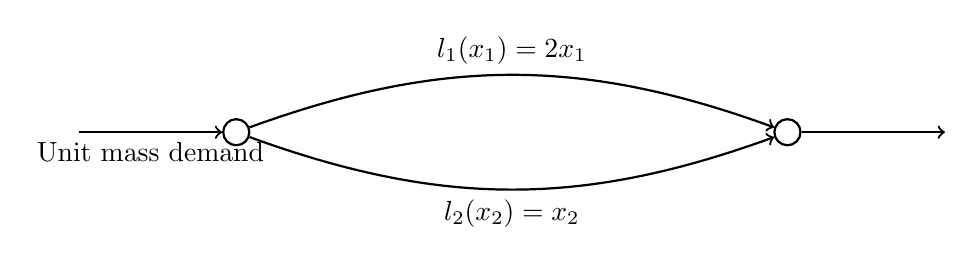
\begin{tikzpicture}
            \begin{scope}[every node/.style={circle,thick,draw}]
                \node (A) at (0,0) {};
                \node (B) at (7,0) {};
            \end{scope}
            \begin{scope}[every path/.style={->,thick}]
                \path [->] (-2,0) edge node[midway, below]{Unit mass demand}(A);
                \path [->] (A) edge [bend left=20] node[midway, above]{$l_1(x_1)=2x_1$}(B);
                \path [->] (A) edge [bend right=20] node[midway, below]{$l_2(x_2)=x_2$}(B);
                \path [->] (B) edge (9,0);
            \end{scope}
        \end{tikzpicture}
    \end{center}
    Suppose we have a unit mass of traffic going through two routes with $l_1$ or $l_2$ cost each. We find the nash equilibrium subject to $x_1+x_2=1$, $x_1,x_2\geq 0$. 
\end{aexample}
This is very intuitive. Relating $l_1(x_1)=l_2(x_2)$ gives $x_1=1/3,x_2=2/3$.
\begin{remark}
    This is also known as a \textbf{wardrop equilibrium}. The cost on all the paths used is the same. The cost on all the paths that are not used is greater than on the used paths.
\end{remark}

\begin{aexample}{Pigon}{pigon}
    Consider the following `traffic diagram'.
    \begin{center}
        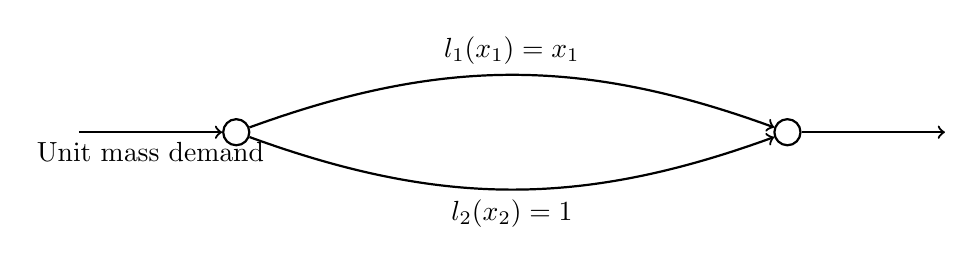
\begin{tikzpicture}
            
        \begin{scope}[every node/.style={circle,thick,draw}]
            \node (A) at (0,0) {};
            \node (B) at (7,0) {};
        \end{scope}
        \begin{scope}[every path/.style={->,thick}]
            \path [->] (-2,0) edge node[midway, below]{Unit mass demand}(A);
            \path [->] (A) edge [bend left=20] node[midway, above]{$l_1(x_1)=x_1$}(B);
            \path [->] (A) edge [bend right=20] node[midway, below]{$l_2(x_2)=1$}(B);
            \path [->] (B) edge (9,0);
        \end{scope}
        \end{tikzpicture}
    \end{center}
\end{aexample}
The wardrop equilibrium here is $x_1=1,x_2=0$. 
This is interesting, as we can consider the social cost, defined as the expected value of the cost for the players. In this case, everyone needs to pay a cost of $1$.

However, let us suppose that there is a planner who would like to minimize this total cost \[
\min_{x_1} x_1l(x_1)+x_2l(x_2) = \min x_1^2+(1-x_1).
\]
Completing the square gives a minimal cost when $x_1=1/2$ with a total cost of $3/4$. However, this is not a stable minima. There is an incentive to deviate from the assigned route.
    Let us define the price of anarchy \[
    P \defeq \frac{\textrm{cost with equilibrium}}{\textrm{cost with planner}}.
    \]
$P=1$ is the best outcome. But in this case we have a price of $1/(3/4) = 4/3$.
Consider the following diagram.
\begin{center}
    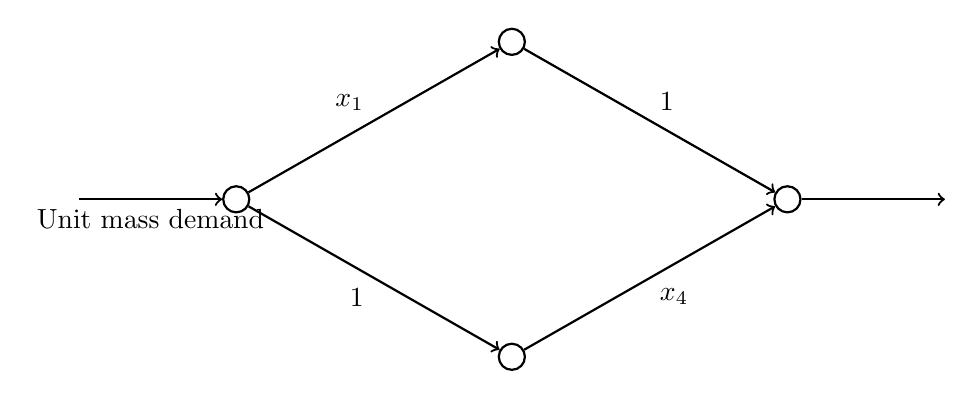
\begin{tikzpicture}
        
    \begin{scope}[every node/.style={circle,thick,draw}]
        \node (A) at (0,0) {};
        \node (B) at (7,0) {};
        \node (C) at (3.5,2){};
        \node (D) at (3.5,-2){};
    \end{scope}
    \begin{scope}[every path/.style={->,thick}]
        \path [->] (-2,0) edge node[midway, below]{Unit mass demand}(A);
        \path [->] (A) edge node[midway, above left] {$x_1$}(C);
        \path [->] (A) edge node[midway, below left] {$1$}(D);
        \path [->] (C) edge node[midway, above right] {$1$}(B);
        \path [->] (D) edge node[midway, below right] {$x_4$}(B);
        \path [->] (B) edge (9,0);
    \end{scope}
    \end{tikzpicture}\end{center}

Now, the equilibrium is when $x_1=x_4=1/2$, with a total social cost of $3/2$.
    Suppose we now create a new road.

    \begin{center}
        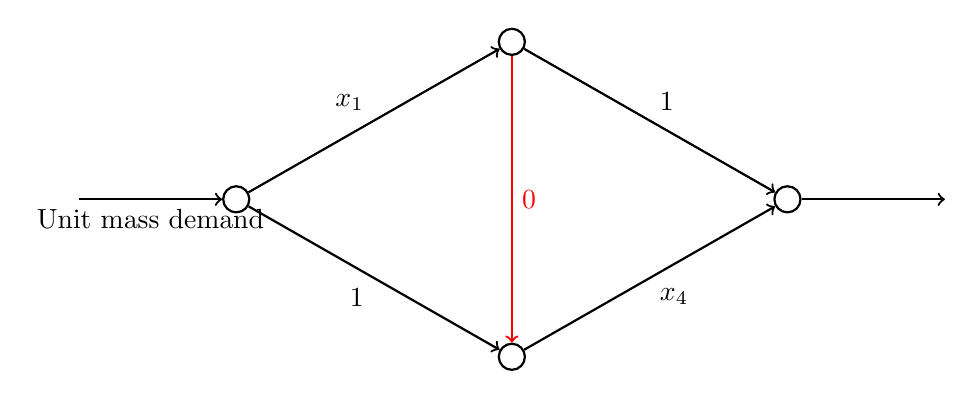
\begin{tikzpicture}
            
        \begin{scope}[every node/.style={circle,thick,draw}]
            \node (A) at (0,0) {};
            \node (B) at (7,0) {};
            \node (C) at (3.5,2){};
            \node (D) at (3.5,-2){};
        \end{scope}
        \begin{scope}[every path/.style={->,thick}]
            \path [->] (-2,0) edge node[midway, below]{Unit mass demand}(A);
            \path [->] (A) edge node[midway, above left] {$x_1$}(C);
            \path [->] (A) edge node[midway, below left] {$1$}(D);
            \path [->] (C) edge node[midway, above right] {$1$}(B);
            \path [->] (D) edge node[midway, below right] {$x_4$}(B);
            \path[red](C)edge node[midway, right]{$0$}(D); 
            \path [->] (B) edge (9,0);
        \end{scope}
        \end{tikzpicture}\end{center}

Now, the best road is to go up then through the red edge. This means the new equilibrium now is $x_1=x_4=1$ with a total social cost of $2$. This is known as \textbf{Braess's paradox}, where adding more resources to the system causes the social cost to increase.

\subsection*{Existence of Wardrop Equilibria}.
We want to determine when wardrop equilibria exist in the following graph.

\begin{center}
    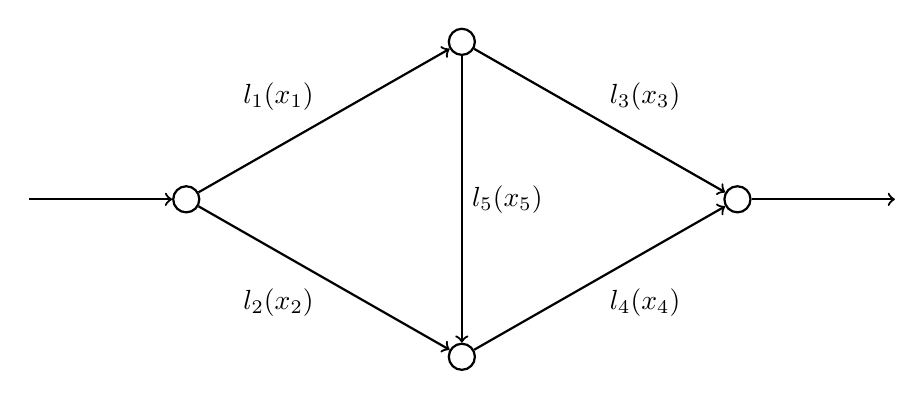
\begin{tikzpicture}
        
    \begin{scope}[every node/.style={circle,thick,draw}]
        \node (A) at (0,0) {};
        \node (B) at (7,0) {};
        \node (C) at (3.5,2){};
        \node (D) at (3.5,-2){};
    \end{scope}
    \begin{scope}[every path/.style={->,thick}]
        \path [->] (-2,0) edge (A);
        \path [->] (A) edge node[midway, above left] {$l_1(x_1)$}(C);
        \path [->] (A) edge node[midway, below left] {$l_2(x_2)$}(D);
        \path [->] (C) edge node[midway, above right] {$l_3(x_3)$}(B);
        \path [->] (D) edge node[midway, below right] {$l_4(x_4)$}(B);
        \path(C)edge node[midway, right]{$l_5(x_5)$}(D); 
        \path [->] (B) edge (9,0);
    \end{scope}
\end{tikzpicture}\end{center}
\begin{atheorem}{}{}
    Assume that each $l_i(x_i)$ is non-negative, non-decreasing, and differentiable. Then a unique Wardrop Equilibrium exists.
\end{atheorem}
\begin{proof}[Sketch of proof]
    Let $P$ be the set of all paths from the source to the destination.
    Let $x_p$ be the number of users on path $i$, and $E$ be the set of edges. We now have an optimization \[
        \min_{\{x_p:p\in P\} } \sum_{i\in E} \int_{0}^{\textrm{total traffic on $i$}} l_i(z) dz
    \]
    subject to $\sum_{p\in P} x_p=1, x_p\geq 0 \forall p\in P$.

    We claim that this optimization problem has a unique solution, and this solution is the Wardrop equilibrium. The argument boils down to showing that the function is convex,thus has a unique minimum. 

    Let $\lambda$ be a Lagrange Multiplier for the condition $\sum_{p\in P} x_p=1$. Then the first order optimality shows that \[
    \sum_{\textrm{edges in path $p$}} l_i(\sum_{\textrm{paths $p$ using $i$}}x_p)\geq \lambda
    \]
    with equality when $\sum {x_p}>0$.
\end{proof}

\section{Lecture 5: Pricing}
\newsection
\subsection*{Recap}
\begin{enumerate}
    \item Zero sum games
    \item Infinite population games - non-atomic traffic flow games.
\end{enumerate}
Recall in the last lecture we had in example \ref{pigon}:
\begin{center}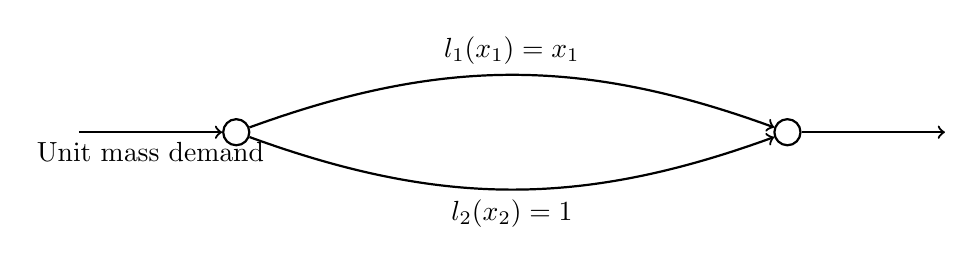
\begin{tikzpicture}
            
    \begin{scope}[every node/.style={circle,thick,draw}]
        \node (A) at (0,0) {};
        \node (B) at (7,0) {};
    \end{scope}
    \begin{scope}[every path/.style={->,thick}]
        \path [->] (-2,0) edge node[midway, below]{Unit mass demand}(A);
        \path [->] (A) edge [bend left=20] node[midway, above]{$l_1(x_1)=x_1$}(B);
        \path [->] (A) edge [bend right=20] node[midway, below]{$l_2(x_2)=1$}(B);
        \path [->] (B) edge (9,0);
    \end{scope}
    \end{tikzpicture}
\end{center}
Which had conflicting social optimal and equilibrium. However, we can introduce a price of $t_1=1/2$ to the upper route. i.e. $l_1(x_1)=x_1+1/2$ In this case, the equilibrium is when $x_1=x_2=1/2$. From an observer standpoint, we can disregard the tolls and get the social optimum strategy. However, for the drivers' standpoint, they still incur the full cost of $1$.

From an economic standpoint, we can disregard the cost of the toll. This is because the planner gets the toll fee of $(1/2)(1/2)=1/4$, but then this can be redistributed to everyone. 
\begin{remark}
    You can think of it `transfering' part of the cost of the bottom road to the top road to have $3/4$ cost each.
\end{remark}

We revisit the original model without tolls. Suppose that $x_1$ drivers are taking the top road and we consider the next driver ($x_1+\epsilon$?).

We define the social cost of the driver taking the top road as \[
\frac{d}{dx_1}x_1l_1(x_1)= x_1l_1'(x_1)+l_1(x_1).
\]
Previously each driver in the selfish equilibrium compares the costs $l_1(x_1)$ and $l_2(x_2)$. This is the second term in the cost. The first term is called \textbf{externality}.
\begin{atheorem}{Pigovian tax}{}
    Let $\tilde{l}_j(x)=xl_j'(x)+l_j(x)$. Under the new graph with costs $\tilde{l}_j$, the Wardrop eqiulibrium is the social optimal strategy with original costs.
\end{atheorem}
\corollary{
    The optimal toll cost for each road is $xl'(x)$. (up to a constant difference, but that is redistributed anyway.)
}

\subsection*{Finite number of users}
These leads to models that are known as congestion games. (Rosenthal, 1973)
\begin{remark}
    Rosenthal studied IEMS in Northwestern.
\end{remark}
\definition{Congestion Game}{
    A \textbf{congestion game} is a game with\begin{itemize}
        \item A set of players $R=\{1,2,\ldots,n\}$
        \item A set of resources $M=\{1,2,\ldots,m\}$
        \item For each $i\in R$, a set $S_i\subseteq M$ denoting the set of resources $i$ can use.
        \item Each resource has a cost of $c^j(x_j)$, where $x_j$ is the total number of players using the resource. The cost for player $i$ is $c_i(s_i,s_{-i})=\sum_{j\in s_i}c^j(x_j)$.
    \end{itemize}
}
\begin{aexample}{}{}
    
\begin{center}
    \begin{tikzpicture}
        
    \begin{scope}[every node/.style={circle,thick,draw}]
        \node [label=below:{player 1}](A) at (0,0) {};
        \node (B) at (7,0) {end};
        \node (C) at (3.5,2){};
        \node (D)[label=below:{player 2}] at (3.5,-2){};
    \end{scope}
    \begin{scope}[every path/.style={->,thick}]
        \path [->] (-2,0) edge (A);
        \path [->] (A) edge node[midway, above left] {$1$}(C);
        \path [->] (A) edge node[midway, below left] {$4$}(D);
        \path [->] (C) edge node[midway, above right] {$2$}(B);
        \path [->] (D) edge node[midway, below right] {$5$}(B);
        \path [->] (B) edge (9,0);
        \path [->] (D) edge node[midway, below right] {$3$}(C);
    \end{scope}
    \end{tikzpicture}\end{center}

Consider this game where both players want to reach the end.The roads are numbered 1 to 4. We have \begin{align*}
    M=&\{1,2,3,4,5\},\\
    S_1=&\{(1,2),(4,5),(4,3,2)\},\\
    S_2=&\{(3,2),5\}.
\end{align*}

\end{aexample}
\begin{aexample}{El Farol Bar Problem}{}
    10 people decide to go to the bar or go home. 
    If 6 or fewer go they have more fun than staying home. If 7 or more go, the bar is too crowded and they have less fun.
\end{aexample}
How do we model this as a congestion game?
We can model the resources as \[
\{\rm{bar}, \rm{home}\}.
\]
The strategy set of each player is \[
S_i=\{\rm{bar},\rm{home}\}
\]
Under this, the payoff is\[
\pi_i(s_i)=\begin{cases}
    1,&\textrm{if $x_{\rm{bar}}\leq 6$ and $s_i=$bar}\\-1,&\textrm{if $x_{\rm{bar}}\geq 7$ and $s_i=$bar}\\
    0,&\textrm{if $s_i=$home}\\
\end{cases}
\]
\begin{atheorem}{Rosenthal}{}
    Every congestion game has a pure strategy Nash equilibirum.
\end{atheorem}
We will \hyperref[]{prove this result} later.
\definition{Potential Game}{
    A game $G=(R,\{S_r\},\{\pi_r\})$ is a \textbf{potential game} if there is a function \[
    P:\prod_{r\in R} S_r\to \reals
    \]
    such that for all $r\in R$, $\bar{s}_{-r}$, and $x,z\in S_r$,
    \[
        \pi_r(x,\bar{s}_{-r})-\pi_r(z,\bar{s}_{-r})\geq 0 \iff P(x,\bar{s}_{-r})-P(z,\bar{s}_{-r})\geq 0
    \]
    with equality on the left iff equality on the right.
    In this case, we call $P$ a(an) \textbf{(ordinal) potential}.
    If \[
        \pi_r(x,\bar{s}_{-r})-\pi_r(z,\bar{s}_{-r})= P(x,\bar{s}_{-r})-P(z,\bar{s}_{-r}),
    \]
    we can $P$ an \textbf{exact potential}.
}
That is, a player benefits from changing strategies if and only if they can increase the potential.

Potential games exist.
\begin{aexample}{Cournot competition potential}{}
    $R$ firms choose $q_i\in[\epsilon,q_{\rm{max}}]$. The payoff for each company is \[
    \pi_i = q_i(P(Q)-c)
    \]
    where $Q=\sum q_r$.
    We let \[
        \Psi(q_1,\ldots, q_R) = \left(\prod_r q_r \right)(P(Q)-c).
    \]
    Then \begin{align*}
        \Psi(q_i,\bar{q}_{-i})-\Psi(\tilde{q}_i,\bar{q}_{-i})=&\left(\prod_{r\neq i}q_r\right)(q_i(P(Q_{-i}+q_i)-c)-\tilde{q}_i(P(Q_{-i}+\tilde{q}_i)-c))\\
        =&\left(\prod_{r\neq i}q_r\right)(\pi_i(q_i,\bar{q}_{-i})-\pi_i(\tilde{q}_i,\bar{q}_{-i})).
    \end{align*}
    This is \textit{almost} a potential game for $q_i\in[0,q_{\rm{max}}]$. Stricter conditions on $P$ can give potentials. 
\end{aexample} 

\begin{alemma}{}{}
    Every congestion game is a potential game
\end{alemma}

\begin{proof}[Sketch]
    We need to construct a potential for the congestion game. We claim \[
    P(\bar{s})= \sum_{j\in M}\sum_{1}^{x_j}C^j(k) 
    \]is a potential.
    Intuitively, take each resource $j$, then sum $C^j$ all the way from $1$ user to $x_j$ users.

    Suppose user $i$ using one $s_i$ and wants to switch towards using $\tilde{s}_i$. The change in cost is \[
        \pi_i(s_i,\bar{s}_{-i})-\pi_i(\tilde{s}_i,\bar{s}_{-i})=C^{s_i}(x_{s_i})-C^{\tilde{s}_i}(x_{s_i}).
    \]
    This is exactly the change in potential. (Apply an inductive argument).
\end{proof}
\begin{atheorem}{}{}
    Every potential game has a Nash equilibrium if the potential obtains its maximum for some strategy profile.
\end{atheorem}
\begin{proof}
    There is a maximal value for the potential function. Each player picks the strategy that maximize this potential function. This must be a Nash equilibirum.
\end{proof}
\corollary{
    Every finite potential game has at least one pure strategy Nash equilibrium. 
    Every game with a compact strategy set has at least one pure strategy Nash equilibrium.
}

\begin{proof}[Proof of Rosenthal]
    A congestion game has finite players and finite resources. Therefore it is a finite game. Since all congestion games are potential games, we are done.
\end{proof}


Nash equilibriums can be reached by using best response in potential games. I.e. choose one player and change his strategy to be the best response. The potential is strictly increasing, so has to be reached at some point. 
\section{Lecture 6: Best Response Dynamics}
\newsection
\subsection*{Recap}
\begin{enumerate}
    \item Pigovian tax
    \item Congestion games
    \item Potential game
\end{enumerate}

\definition{Sequential Best Response Dynamics}{
    Given a game $G$. We consider the following algorithm:
    \begin{itemize}
        \item set $k=0$
        \item pick an initial profile $(s_1^0,\ldots,s_R^0)$
        \item pick one player $i$, update $s_i^{k+1}\in B_i(\bar{s}_{-i}^k)$. 
        \item For every $j\neq i$ set $s_j^{k+1}=s_j^k$.
        \item This is the new strategy profile. $k+=1$ and repeat.
    \end{itemize}
}

\proposition{If this converges, we have a Nash Equilibrium.}

\example{
    Consider the game with the following payoff:
    \begin{center}
        
    \begin{tabular}{|c| c c c|} 
        \hline
        1\textbackslash 2&L & M & R\\
        \hline
      U& (10,10) & (2,2) & (1,1)\\
       \hline
      M& (7,8) & (6,3) & (5,9)\\
       \hline
      D& (6,6) & (5,2) & (8,4)\\
       \hline
    \end{tabular}
    \end{center}
    Starting from (M,M), we alternate between players 1 and 2 for best response to go to (M,R), (D,R), (D,L), (U,L), which is the Nash equilibrium.
}
In general, this forms a directed graph with $R \# \textrm{number of states}$ edges. So this is the bound on the number of iterations. If you have $N$ players and $2$ strategies each, you can have $N2^N$ iterations.


\example{
    Consider the game with the following payoff:
    \begin{center}
        
    \begin{tabular}{|c| c c c|} 
        \hline
        1\textbackslash 2&L & M & R\\
        \hline
      U& (10,10) & (0,0) & (0,0)\\
       \hline
      M& (0,0) & (0,1) & (1,0)\\
       \hline
      D& (0,0) & (1,0) & (0,1)\\
       \hline
    \end{tabular}
    \end{center}
    We embedded the attacker defender payoff in the payoff, so this is actually a loop; no way to leave to get the Nash equilibrium. 
}

\definition{Parallel Best Response}{
    We consider the the best response dynamic, except for all $i$, we update $s_i^{k+1}=B_i(\bar{s}_{-i}^k)$ simutaneously.
    
} 

\example{
    This is not guaranteed to converge (even if iteratively the sequential best response dyanmic gives convergence).
    The game with payoff \begin{center}
        
        \begin{tabular}{|c c|} 
            \hline
            (10,10)&(0,0)\\
            \hline (0,0)&(10,10)
            \\ \hline
        \end{tabular}
        \end{center}
    does not converge with parallel response dynamic if you start in the wrong corner.
}

\begin{aexample}{Cournot competition convergence}{}
    \begin{center}
        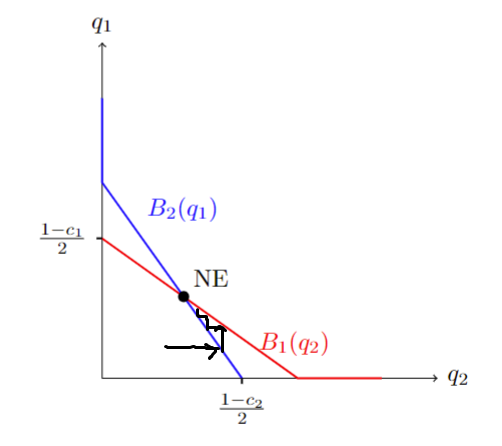
\includegraphics{cournot convergence.png}
    \end{center}
\end{aexample}
However, if we swap 
\begin{center}
    
\begin{tikzpicture}[scale=4, every node/.style={font=\small}]
    % Axes
    \draw[->] (0,0) -- (1.2,0) node[right] {$q_2$};
    \draw[->] (0,0) -- (0,1.2) node[above] {$q_1$};
    
    % Best response lines
    \draw[red, thick] (0,0.7) -- (0.5,0) node[pos=0.75, below left] {$B_1(q_2)$} -- (1,0);
    \draw[blue, thick] (0.7,0) -- (0,0.5) node[pos=0.75, above right] {$B_2(q_1)$}--(0,1);

    % Nash equilibrium point
    \fill (0.291667,0.291667) circle (0.02) node[above right] {NE};

    % Labels on axes
    \draw[thick] (0,0.7) -- (-0.02,0.7) node[left] {$\frac{1-c_1}{2}$};
    \draw[thick] (0.7,0) -- (0.7,-0.02) node[below] {$\frac{1-c_2}{2}$};
\end{tikzpicture}

\end{center}
The middle nash equilibrium point becomes unstable and the ends become stable.

\definition{Stable and unstable equilibria}{
    We call the equilibrium stable best response dynamic converges to the equilibrium and unstable otherwise.
}
\definition{Strategic complements}{
    This refers to a game where the value of a given action increases as other agents take that action.
}
\begin{aexample}{Language game}{}
    We have $N$ people and two languages, French and English. The payoff of choosing a language is equal to the number of people choosing the language. 
\end{aexample}


\begin{aexample}{Power control}{}
    There are $2$ transmitters. Each transmitter chooses the power level $P_i\in[0,1]$. The payoff function \[
    \pi_i(P_i,P_{-i}) = \begin{cases}
        1-cP_i, &\textrm{if $\frac{P_i}{P_{-i}+N}>\gamma$}\\
        0, &\textrm{otherwise}.
    \end{cases}
    \]With $c$ chosen to be small enough that it is interesting.
\end{aexample}

\definition{Increasing differences}{
    Let $X\subseteq \reals$, and $T$ a partially ordered set. Then $f:X\times T\to \reals$ has \textbf{increasing differences} if $
    \forall x'\geq x, t'\geq t   
    $\[
    f(x',t')-f(x,t')\geq f(x,t)-f(x,t).
    \]
}
\begin{remark}
    If $T\subseteq \reals^k$ (partial order is $\geq$ in every entry of the vector) and $f$ is $C^2$, this condition is equivalent to \[
        \frac{\partial^2 f}{\partial x \partial t_i}\geq 0
    \]
    for all $x$, $t_i$.
\end{remark}

\theorem{Topkis}{
    Let $X\subseteq \reals$ compact and $T$ partially ordered. Let $f:X\times T\to \reals$ be continuous in $X$ and has increasing differences. Then \begin{itemize}
        \item $x(t) \defeq \arg\max_{x\in X} f(x,t)$ is non-empty.
        \item $x(t)$ has a largest and smallest element $\bar{x}(t)$ and $\underline{x}(t)$ respectively.
        \item  $\bar{x}(t)$ and $\underline{x}(t)$ are increasing in $t$.
    \end{itemize} 
}
\begin{proof}
    The first two statements are a consequence of continuity and compactness, and the extreme value theorem.
    The last statement probably uses some kind of measure theory.
\end{proof}

\definition{Super Modularity}{
    A game $G=\{R,\{S_r\},\{\pi_r\}\}$ is \textbf{supermodular} if for all $r\in R$,\begin{itemize}
        \item $S_r$ is a compact subset of $\reals$.
        \item $\pi_r$ is continuous in $s_i$ and $s_{-i}$
        \item $\pi_r$ has increasing differences in $s_i,\bar{s}_{-i}$.
    \end{itemize}

}
\begin{remark}
    This is not the most general definition. But this is good enough.
\end{remark}
Given a supermodular game, we get that the best response $B_i\defeq \arg\max_{s_i\in S_i}\pi_i(s_i,\bar{s}_{-i})$ is non empty, has a largest and smallest element $\bar{B}_i$, $\underline{B}_i$, and these are increasing in $\bar{s}_{-i}$.
This captures the idea of complementarity. If other agents increase their strategies, the best response is to also increase. 

\begin{aexample}{}{}
    Let $s^0=(s_1^0,\ldots, s_R^0)$ where $s_i^0$ is the largest element in $S_i$. Starting here, we run parallel best response using $\bar{B}_i$ for all $i$. We show that this converges to a Nash equilibrium.
\end{aexample}
\begin{proof}
    We show that $s^k\leq s^{k-1}$ for all $k$. Then, by MCT, this converges to a Nash equilibrium. To show this, we proceed by induction. 
    The case $s^1\leq s^0$ is trivial by the definition of $s^0$.
    Then if $s^{k-1}\leq s^k$, then \[
    s_i^{k+1}=\bar{B}_i(s^k_{-i}) \leq \bar{B}_i(s^{k-1}_{-i}) = s_i^k
    \]
    by Topkis's theorem. 
\end{proof}
\begin{remark}
    We can also start from the smallest element, then work our way up to a (possibly different) Nash equilibrium. If all the strategy sets are intervals, we can consider the box that has the two vertices with the two Nash equilibria. It is not hard to see that any other Nash equilibrium has to be inside the box, by the increasing difference property. Hence, if the two equilibria are the same there is a unique equilibria.
\end{remark}
\begin{aexample}{Betrand Competition}{}
    We have $N$ firms, each firm chooses their price $p_i$. The demand for firm $i$ is \[
    D_i (p_i,\bar{p}_{-i})=a_i-b_ip_i+\sum_{j\neq i} d_{ij} p_j,
    \]where $a_i,b_i,d_{ij}\geq 0$.
    The payoff of the firm is \[
    \pi_i(p_i,\bar{p}_{-i})=p_iD_i(p_i,\bar{p}_{-i}).
    \]
    Then we have \begin{align*}
    \frac{\partial \pi_i}{\partial p_i} &= a_i-2b_ip_i+\sum_{j\neq i} d_{ij} p_j,\\
    \frac{\partial \pi_i}{\partial p_i\partial p_j} &= d_{ij} \geq 0.
    \end{align*}
    Subject to some technicalities on the prices the firms can choose, this is a supermodular game. 
\end{aexample}
\usection{Lecture 7: Fictitious play}
\newsection
\subsection*{Logistics}
\begin{itemize}
    \item Posted project description
    \item HW will be posted tonight
\end{itemize}
\subsection*{Recap}
\begin{enumerate}
    \item Best response dynamics
    \item Supermodular games 
\end{enumerate}

The idea of fictitious play is that each player assumes the opponents are using a `stationary mixed strategy'.
Instead of best response to last action, we estimate the mixed strategy and respond to the estimated strategy.
\definition[]{}{
    Let $\{G_t\}_{t\in\mathbb{N}}$ be a sequence of the same games (i.e same players) indexed in $t$ (and played in this order). Let $S_i^t$ be the (pure) action of player $i$ at time $t$. Let $\gamma_i^t(s_i)$ be the count $\#\{s_i^{t'<t}=s_i\}$.
    Therefore, we can approximate the probability distribution \[
    p_i^t(s_i)=\frac{\gamma_i^t(s_i)}{t}.
    \]
    Each player in fictitious play chooses $s_i^t\in B_i(\bar{p}_{-i}^t)$.
}
\begin{remark}
    The trajectory is not unique.
\end{remark}
\begin{remark}
    At $t=0$ we can assume that the strategy is arbitrary, or each player has an initial `belief' of the other agents' mixed strategies and update accordingly.
\end{remark}
\begin{aexample}{}{}
    Consider the game with payoff
    \begin{center}
       
        \begin{tabular}{|c|c c|} 
            \hline &L & R\\
            
            \hline
            U&(3,3)&(0,0)\\
            \hline D&(4,0)&(1,1)
            \\ \hline
        \end{tabular}
        \end{center}
        There is a Nash equilibrium of (1,1). The game progresses as 
        \begin{center}
       
            \begin{tabular}{|c|c c c|} 
                \hline 
                $t=0$ & $p_1(U,D)$&$p_2(L,R)$& $(U,L)$\\
                \hline $t=1$ & (1,0) & (1,0) & $(D,L)$\\
                \hline
                $t=2$ & (1/2,1/2) & (1,0) & $(D,L)$\\
                \hline 
                $t=3$ & (1/3,2/3) & (1,0) & $(D,L)$
                \\
                \hline 
                $t=4$ & (1/4,3/4)& (1,0)  & $(D,R)$\\ \hline
            \end{tabular}
            \end{center}
            And $(D,R)$ continues after $t>4$.
\end{aexample}

This equilibrium is found without requiring knowledge of the other's payoffs.

\definition{Convergence of strategy profiles}{
    A sequence of strategy profiles $\{\bar{s}^t\}$ \textbf{converges} to  a profile $\bar{s}$ if there exists $T$ such that $\bar{s}^t=\bar{s}$ for all $t\geq T$. We denote this $\bar{s}^t\to \bar{s}$.
}
\proposition{
    Under fictitious play, 
    \begin{enumerate}
        \item A strategy profile that converges must converge to a pure strategy Nash Equilibrium.
        \item If for some time $T$, $\bar{s}^T=\bar{s}^*$, a strict Nash equilibrium, then $\bar{s}^t=\bar{s}^*$ for all $t>T$.
    \end{enumerate}   
}
\begin{proof}
    For the first statement, we play the game enough so that the empirical probability distribution concentrates approaches a pure strategy. Then by definition this is a pure strategy Nash equilibrium.

    For the second statement, 
    we note that \begin{align*}
    p_i^{T+1}(s_i)&=\frac{\gamma_i^T(s_i)+ I_{s_i=s_i^*}}{T+1}\\
    &= (1-\alpha)p_i^T(s_i)+\alpha I_{s_i=s_i^*},
    \end{align*}
    where $\alpha = t/(t+1)$.
    That means the new distribution is a convex (linear) mixture of the previous distribution and the Nash equilibrium.
    But for the Nash equilibrium and the previous distribution, the best response is $s_i^*$ for each player $i$. Since the best response for the Nash equilibrium has a strict inequality, we can conclude that the best response for time $T+1$ must also lead to the Nash equilibrium. Inductively, the strategy profile has to be the Nash equilibrium for all $t>T$.
\end{proof}

\definition{Convergence of Empirical Beliefs}{
We say that $\{\bar{s}^t\}$ converges to $\sigma$ in the time average sense if \[
\lim_{t\to \infty} p_i^t(s_i)=\sigma(s_i)
\]
for all $i$ and $s_i\in S_i$.
}
\example{
    For the \hyperref[ex:attackdefend]{attacker defender problem}, we can show that this converges to $(1/2,1/2)$ for each player.
    \begin{center}
    \begin{tabular}{|c|c c c|} 
        \hline 
        $t=0$ & $p_1(A,B)$&$p_2(A,B)$& $(A,A)$\\
        \hline $t=1$ & (1,0) & (1,0) & $(A,B)$\\
        \hline
        $t=2$ & (1,0)& (1/2,1/2) & $(B,B)$\\
        \hline 
        $t=3$ & (2/3,1/3) & (1/3,2/3) & $(B,A)$
        \\
        \hline 
        $t=4$ & (1/2,1/2)& (1/2,1/2)  & $(A,A)$\\ \hline
    \end{tabular}
    \end{center}
    and the cycle repeats. 
    The empirical beliefs converges to (1/2,1/2), (1/2,1/2).
}

\theorem[]{}{
    Suppose that fictitious play converges in time average to $\sigma$. Then $\sigma$ is a mixed-strategy Nash equilibrium.
}
\theorem[]{}{
    Fictitious play converges in time average for \begin{enumerate}
        \item A two player zero-sum game.
        \item A two player game with at most two strategies for each player.
        \item A game that is solvable by iterated strict dominance.
        \item A potential game. 
        \item Some supermodular games. 
    \end{enumerate}
}
\begin{aexample}{Miscoordination}{}
    Consider the game with payoff matrix
    \begin{center}
       
        \begin{tabular}{|c|c c|} 
            \hline &A & B\\
            
            \hline
            A&(1,1)&(0,0)\\
            \hline B&(0,0)&(1,1)
            \\ \hline
        \end{tabular}
        \end{center}

    There is a mixed strategy equilibrium where the players choose $A$ and $B$ with half probability each.
    There is a sequence 
    \begin{center}
        \begin{tabular}{|c|c c c|} 
            \hline 
            $t=0$ & $p_1(A,B)$&$p_2(A,B)$& $(A,B)$\\
            \hline $t=1$ & (1,0) & (0,1) & $(B,A)$\\
            \hline
            $t=2$ & (1/2,1/2)& (1/2,1/2) & $(A,B)$\\
            \hline 
            $t=3$ & (1/3,2/3) & (2/3,1/3) & $(B,A)$
            \\
            \hline 
            $t=4$ & (1/2,1/2)& (1/2,1/2)  & $(A,B)$\\ \hline
        \end{tabular}
        \end{center}
        In the limit, this indeed gives us the time average empirical beliefs. However, they are not getting the correct payoffs. (0 each time).
\end{aexample}
\begin{aexample}{Non-convergence}{}
    Consider the game with the reward matrix  \begin{center}
       
        \begin{tabular}{|c|c  c c|} 
            \hline &R & P & S\\
            
            \hline
            R&(0,0)&(1,0)&(0,1)\\
            \hline P&(0,1)&(0,0)&(1,0)\\
             \hline S&(1,0)&(0,1)&(0,0)
            \\ \hline
        \end{tabular}
        \end{center}
The unique Nash equilibirum is $(1/3,1/3,1/3)$.
The sequence here starts with everyone best responding (R,S), (R,P), (S,P), (S,R), (P,R), (P,S), (R,S). Then the cycle length increases (R,S), (R,P), (R,P), (S,P), (S,P)...

So this does not converge (cycle lengths are too long).
\end{aexample}
\section{Lecture 8: Evolutionary Game Theory}
\newsection
\subsection*{Logistics}
\begin{itemize}
    \item HW2 posted, due one week from today.
\end{itemize}

Evolutionary Game Theory dates back to 1973 (John Maynard Smith, George Price).

The idea is that we have a large population of potential players. For instance, different species/phenotypes of individuals. We pick two agents from this population to play a game. The winner reproduces faster. 

\definition{Evolutionary game theory terminology}{
    Let $G=(\{1,2\},\{S_1,S_2\},{\pi_1,\pi_2})$ be a finite, symmetric game (i.e. $S_1=S_2=S, \pi_1=\pi_2=\pi$). The \textbf{fitness} of a player playing strategy $s_i\in S$ is the expected payoff against a random member of the population.\\
    A strategy $s_j$ is said to \textbf{invade} strategy $s_i$ at level $\epsilon\in[0,1]$ if $\epsilon$ of the population is type $j$ and $1-\epsilon$ of the population is type $i$.\\
    An \textbf{evolutionary stable strategy} (ESS) is a strategy $s_i$ if $\exists\bar\epsilon >0$ such that if any other strategy $s_j$ invades at level $\epsilon<\bar\epsilon$, the fitness of type $i<$ the fitness of type $j$.
}
\begin{remark}
    The fitness depends on the distribution of strategy `types'.
\end{remark}
\begin{remark}
    Intuitively, an evolutionary stable strategy can withstand invation of another strategy up to $\bar\epsilon$.
\end{remark}
\begin{aexample}{}{}
    Consider this payoff for beetle sizes. \begin{center}
        \begin{tabular}{|c|c c|} 
            \hline &smol& beeg \\
            
            \hline
            smol&(5,5)&(1,8)\\
            \hline beeg&(8,1)&(3,3)
            \\ \hline
        \end{tabular}
    \end{center}
    Two smol beetles share the food. Beeg beetle takes most of the food. Two beeg beetles fight too much and the food is not as useful.

    With only smol beetles, the fitness is $5$. Now let us introduce $\epsilon>0$ beeg beetles into the population. The smol beetles now have payoff \[
    5(1-\epsilon)+ \epsilon = 5-4\epsilon.
    \]
    But the beeg beetles have payoff \[
    8(1-\epsilon) + 3\epsilon = 8-5\epsilon > 5-4\epsilon
    \]
    for $0\leq\epsilon\leq 1$. Therefore, being smol is not an evolutionary stable strategy.

    We change variables $\epsilon\mapsto 1-\epsilon$ to see that being beeg is an evolutionary stable strategy.
\end{aexample}
\proposition{
    An evolutionary stationary strategy is a Nash Equilibrium.
}
\begin{proof}
    Suppose a strategy $s^*$ is an evolutionary stable strategy, then \[
        (1-\epsilon)\pi(s^*,s^*)+\epsilon \pi(s^*,s')>
        (1-\epsilon)\pi(s',s^*)+\epsilon\pi(s',s')
        \]
        for some $\epsilon$ small enough and all $s'\neq s^*$.
        Now we take $\epsilon\to 0 $,\[
            \pi(s^*,s^*)\geq\pi(s',s^*).
        \]
\end{proof}
\begin{remark}
    If the Nash equilibrium is weak, then the other inequality is strict:\[
        \pi(s^*,s')>
       \pi(s',s')
    \]
\end{remark}

The converse is also true, a strict nash equilibrium is an evolutionary stable strategy. \[
\textrm{Strict Nash} \subset \textrm{ESS} \subset {Nash}
\]
These are distinct sets.\begin{aexample}{ESS but not strict}{}
    \begin{center}
        \begin{tabular}{|c|c c|} 
            \hline &A& B \\
            
            \hline
            A&(0,0)&(6,0)\\
            \hline B&(0,6)&(3,3)
            \\ \hline
        \end{tabular}
    \end{center}
    There is a weak Nash equilibirum (A,A). But this is an evolutionary stable strategy. \[
    (1-\epsilon)(0)+\epsilon(6)> (1-\epsilon)(0) + \epsilon(3).
    \]
    The reasoning is that adding in $B$ benefits $A$.
\end{aexample}
\begin{aexample}{Nash but not ESS}{}
    \begin{center}
        \begin{tabular}{|c|c c|} 
            \hline &A& B \\
            
            \hline
            A&(4,4)&(0,4)\\
            \hline B&(4,0)&(3,3)
            \\ \hline
        \end{tabular}
    \end{center}
    There is a weak Nash equilibirum (A,A). But this is an not an evolutionary stable strategy. \[
    (1-\epsilon)(4)+\epsilon(0)<(1-\epsilon)(4) + \epsilon(3).
    \]
    Adding in any small amount of B to the population of $A$ causes a decrease in payoff.
\end{aexample}
\definition{Mixed evolutionary stable strategy}{
    A mixed strategy $\sigma^*$ is an ESS if there exists $\bar\epsilon > 0$ such that for all $\epsilon<\bar\epsilon$,\[
        \pi_i(\sigma^*,\epsilon\sigma'+(1-\epsilon)\sigma^*)>\pi_i(\sigma',\epsilon\sigma'+(1-\epsilon)\sigma^*),
    \]
    for any other mixed strategy $\sigma'$.
}
\begin{aexample}{Hawk Dove}{hawkdove}
    \begin{center}
        \begin{tabular}{|c|c c|} 
            \hline &D& H \\
            
            \hline
            D&(3,3)&(1,5)\\
            \hline H&(5,1)&(0,0)
            \\ \hline
        \end{tabular}
    \end{center}

    There are two symmetric strong Nash equilibria (D,H) and (H,D). However, these are not candidates for a pure ESS. We find the mixed ESS by letting a strategy $p$ chance of playing $D$ and $(1-p)$ chance of playing $H$. We solve for \[
    p(3)+(1-p)(1)= p(5)+(1-p)0 \implies p=\frac{1}{3}.
    \]
    This is the only candidate for an evolutionary stable strategy. Indeed,for any other strategy playing $(1,1-q)$ invading $(1/3,2/3)$ at level $\epsilon$, the probability of meeting a dove strategy is \[
    r=(1-\epsilon)\frac{1}{3}+\epsilon q
    \]
    The payoffs are \[
        (\pi_i(\sigma^*,\epsilon\sigma'+(1-\epsilon)\sigma^*))-(\pi_i(\sigma',\epsilon\sigma'+(1-\epsilon)\sigma^*)) = \frac{1}{3}r3 + \frac{1}{3}(1-r)1+\frac{2}{3}r3+\frac{2}{3}(1-r)0 -\ldots >0
    \] Just trust me bro. 
\end{aexample}
By the linearity of expectations, \begin{align*}
    &(\pi_i(\sigma^*,\epsilon\sigma'+(1-\epsilon)\sigma^*))-(\pi_i(\sigma',\epsilon\sigma'+(1-\epsilon)\sigma^*)) \\=& \epsilon(\pi(\sigma^*,\sigma')-\pi(\sigma^*,\sigma^*)) + (1-\epsilon)\epsilon(\pi(\sigma',\sigma')-\pi(\sigma',\sigma^*)) 
\end{align*}
Assume that $\sigma^*$ plays all actions with some probability, and that $\sigma^*$ is a Nash equilibrium. Then \[
\pi(\sigma^*,\sigma^*)=\pi(\sigma,\sigma^*),
\]
as a different mixing of the same strategies. Therefore, it suffices to check that \[
    \pi(\sigma^*,\sigma')-\pi(\sigma^*,\sigma^*)>0
\]to see that it is an ESS.

\subsection*{Replicator Dynamics}
\definition[]{Replicator Dynamics}{
    Let $x_i(t)$ be the fraction of type $i$ in the population at time $t$, so that $\sum_i x_i(t)=1$ for all $t$.
    Let $f_i(\bar{x}(t))$ be the fitness of type $i$ at time $t$.
    Under \textbf{replicator dyanmics}, we evolve the system through the differential equation\begin{align*}
        \frac{d}{dt}\frac{x_i}{x_j}=\frac{x_i}{x_j}[f_i(\bar{x}(t))-f_j(\bar{x}(t))].
    \end{align*}
}
\proposition{
Under replicator dynamics,\[
\frac{d}{dt}x_i(t) = x_i(t)[f_i(\bar{x}(t))-\phi(\bar{x}(t))],
\]where\[
\phi(\bar{x}(t))\defeq \sum_j x_j(t) f_j(\bar{x}(t))
\]
is the average fitness of the population at time $t$.
}
\theorem[]{}{
    If $x^*$ is an ESS, then it is asymptotically stable for replicator dynamics.
}
\section{Lecture 9: Dynamic Games}
\newsection
There are different game types. Static or Dynamic, Complete info or incomplete info, perfect info and imperfect info.

\definition{Dynamic Game}{
 Everybody knows what a dynamic game is. You know it when you see it.
}
\begin{aexample}{Entry Game}{}
    A company (A) can enter the market or decide not to enter the market. Another company (B) is incumbent (already in the market) and can decide to cut or hold prices. The payoff matrix is as follows.
    \begin{center}
        \begin{tabular}{|c|c c|}
            \hline
            A\textbackslash B & cut & hold\\
            \hline
            Don't Enter & (0,2) & (0,3)   \\
            \hline Enter & (-1,1),& (1,1) \\  \hline  
        \end{tabular}
    \end{center}
    The Nash equilibrium is Enter and Hold.
\end{aexample}
However, we can model the game using an extensive form representation. Each B represents a subgame. There are two subgames depending on A's action.
\begin{center}
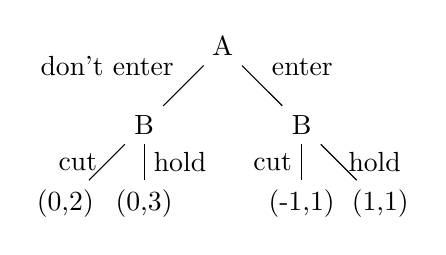
\begin{tikzpicture}
    \node (A) at (0,0){A};
    \node(B) at (-1,-1) {B};
    \node(C) at (1,-1) {B};
    \node(D) at (-2,-2) {(0,2)};
    \node(E) at (-1,-2) {(0,3)};
    \node(F) at (1,-2) {(-1,1)};
    \node(G) at (2,-2) {(1,1)};
    \draw (A) edge  node[midway, above left]{don't enter}(B);
    \draw (A) edge  node[midway, above right]{enter}(C);
    \draw (B) edge  node[midway,  left]{cut}(D);
    \draw (B) edge node[midway,  right]{hold} (E) ;
    \draw (C) edge  node[midway,  left]{cut}(F);
    \draw (C) edge  node[midway,  right]{hold}(G);
\end{tikzpicture}\end{center}
Therefore, we can expand the strategy set of B to be 
\begin{center}
    \begin{tabular}{|c|c c c c|}
        \hline
        A\textbackslash B & (cut, cut) & (cut, hold) &(hold, cut) & (hold, hold) \\
        \hline
        Don't Enter & (0,2) &(0,2)&(0,3)& (0,3)   \\
        \hline Enter & (-1,1),& (1,1)  & (-1,1),& (1,1) \\  \hline  
    \end{tabular}
\end{center}
Therefore, we get a Nash equilibria of (enter, (cut,hold)), (enter, (hold,hold)), (don't enter, (hold,cut)).

However, the first equilibrium is a bit weird. This is because we are implying that B will cut if A doesn't enter. We call this equilibrium \textbf{not sequentially rational}.
\definition{Sequential rationality}{
    A pure strategy Nash equilibrium is said to be \textbf{sequentially rational}, or a \textbf{subgame perfect Nash equilibrium} if the agents' strategies continue to be a Nash equilibrium in every sub game.

}

We can check this using a backward induction algorithm. 
We first consider the strategies B can have at each subgame. If A doesnt enter, then B plays hold. If A enters, it does not matter which one. Now we propagate backwards. If B plays (hold,cut), then A's decision tree is 
\begin{center}
    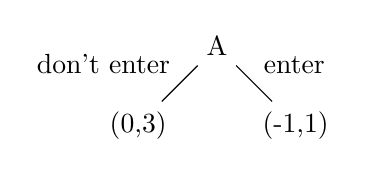
\begin{tikzpicture}
        \node (A) at (0,0){A};
        \node(B) at (-1,-1) {(0,3)};
        \node(C) at (1,-1) {(-1,1)};
        \draw (A) edge  node[midway, above left]{don't enter}(B);
        \draw (A) edge  node[midway, above right]{enter}(C);
    \end{tikzpicture}\end{center}
So (don't enter, (hold,cut)) is a subgame perfect Nash equilibrium.

\begin{atheorem}{}{}
    For a finite dynamic game, the backwards induction algorithm yields exactly all the subgame perfect Nash equilibria.
\end{atheorem}
\begin{aexample}{}{}
    Return to example \ref{ex:attackdefend}.
    \begin{center}
        \begin{tabular}{|c|c c|} 
            \hline
            Attacker\textbackslash User & A&B \\ 
            \hline
            A & (1,0) & (0,1)\\ 
            \hline
            B & (0,1)&(1,0)\\
            \hline
        \end{tabular}
    \end{center}
    We can change this into an extensive form - 
    \begin{center}
        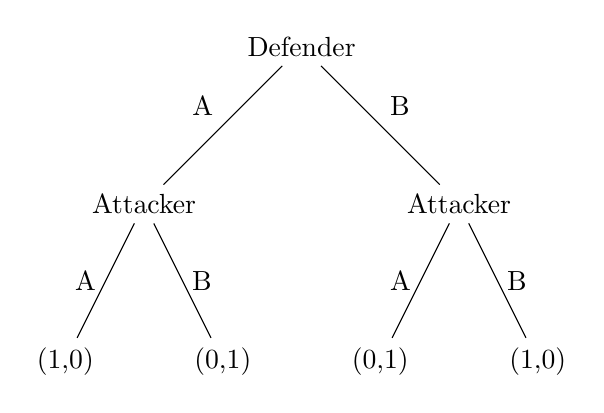
\begin{tikzpicture}
            \node (A) at (0,0){Defender};
            \node(B) at (-2,-2) {Attacker};
            \node(C) at (2,-2) {Attacker};
            \node(D) at (-3,-4) {(1,0)};
            \node(E) at (-1,-4) {(0,1)};
            \node(F) at (1,-4) {(0,1)};
            \node(G) at (3,-4) {(1,0)};
            \draw (A) edge  node[midway, above left]{A}(B);
            \draw (A) edge  node[midway, above right]{B}(C);
            \draw (B) edge  node[midway,  left]{A}(D);
            \draw (B) edge node[midway,  right]{B} (E) ;
            \draw (C) edge  node[midway,  left]{A}(F);
            \draw (C) edge  node[midway,  right]{B}(G);
        \end{tikzpicture}\end{center}
    It is obvious that the attacker has the advantage by choosing the strategy (A,B). The attacker is said to have a \textbf{second mover advantage} as the follower.
\end{aexample}
\begin{aexample}{Stackelberg Competition}{}
    Consider the sequential version of the \hyperref[ex:cournot]{Cournot competition}. Suppose in addition that $c_1=c_2=c\in [0,1]$. Now, let firm 1 plays first, then firm 2.
    Then firm 2's strategy is just to play $B_2(q_1) =  \max\{(1-q_1-c)/2,0\}.$ Naturally we can define $q_2= q_2(q_1)= B_2(q_1).$
    Then $q_1$ is the best response to $q_2$ strategy\[
    B_1(q_2) = \arg\max_{q_1\geq 0} (1-q_1-q_2(q_1))-cq_1. 
\]
solving this yields\[
q_1^*=\frac{1-c}{2},q_2^*=\frac{1-c}{4}.\]
\end{aexample}
Let us compare this to the Nash equilibirum of the static Cournot competition $((1-c)/3,(1-c)/3)$. 
The total quantity produced is \[
3\frac{(1-c)}{4} > 2\frac{(1-c)}{3},
\]
this is good for the consumer because the prices are lower. 
Firm one profits \[
\frac{1-c}{8} > \frac{1-c}{9}.
\]
Form two profits \[
\frac{1-c}{16} > \frac{1-c}{9}.
\]
This game has a first mover advantage. 

\textcolor{red}{TODO: too much work to draw these trees... but you probably understand the concept so whatever}
\begin{aexample}{Three player game}{}
    The outcome at the subgame perfect Nash equilibrium is R,L,R, with a strategy \[
    \{(R,L,(R,R,L))\}.
    \]
\end{aexample}

\begin{aexample}{}{}
    \begin{center}
        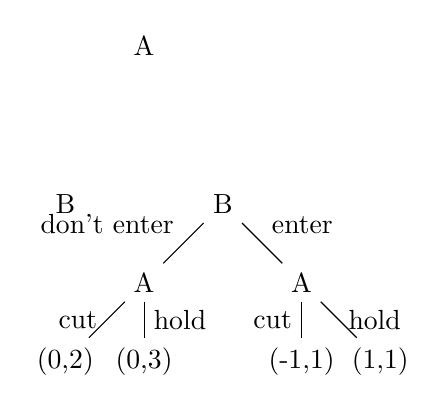
\begin{tikzpicture}
            \node(top) at (-1,2){A};
            \node (ll) at (-2,0) {B};
            \node (A) at (0,0){B};
            \node(B) at (-1,-1) {A};
            \node(C) at (1,-1) {A};
            \node(D) at (-2,-2) {(0,2)};
            \node(E) at (-1,-2) {(0,3)};
            \node(F) at (1,-2) {(-1,1)};
            \node(G) at (2,-2) {(1,1)};
            \draw (A) edge  node[midway, above left]{don't enter}(B);
            \draw (A) edge  node[midway, above right]{enter}(C);
            \draw (B) edge  node[midway,  left]{cut}(D);
            \draw (B) edge node[midway,  right]{hold} (E) ;
            \draw (C) edge  node[midway,  left]{cut}(F);
            \draw (C) edge  node[midway,  right]{hold}(G);
        \end{tikzpicture}\end{center}
\end{aexample}
\section{Lecture 10: }
\newsection
\subsection*{Recap}
\begin{enumerate}
    \item Dynamic (Multi-stage) games.
    \item Game tree (extensive form game)
    \item Sequential rationality - subgame-perfect Nash equilibrium using backward induction.
\end{enumerate}

\begin{aexample}{3 period Bargaining}{}
    Two players are splitting one dollar. 
    They follow an alternating offer bargaining model. The game is terminated when one player accepts.
    
    \begin{itemize}
        \item Period 1: Player 1 makes an offer $(s_1,1-s_1)$. Player 2 can accept or reject the offer.
        \item Period 2: Player 2 makes an offer $(s_2,1-s_2)$. Player 1 can accept or reject.
        \item Period 3: The players get $(s,1-s)$.
    \end{itemize}

    Let $\delta\in(0,1)$. This is the discounted payoff, i.e. how much they discount the future payoff. Therefore, we rewrite it as:
    \begin{itemize}
        \item [1:] Player 1 makes an offer $(s_1,1-s_1)$. Player 2 can accept or reject the offer.
        \item [2:] Player 2 makes an offer $(\delta s_2,\delta(1-s_2))$. Player 1 can accept or reject.
        \item [3:] The players get $(\delta^2 s,\delta^2(1-s))$.
    \end{itemize}
    Work out the SPNE of the game.
\end{aexample}
Using backward induction, for period 2, player 1's response is \[
\begin{cases}
    \rm{accept,} & \textrm{if }\delta s_2\geq \delta^2s\implies s_2\geq \delta s,\\
    \rm{reject,} & \textrm{otherwise.} 
\end{cases}
\]
So player 2 can offer $(\delta s, 1-\delta s)$ with an intention to get $\delta (1-\delta s)$.
Therefore, player 2 rejects player 1's offer in period 1 if \[
1-s_1<\delta (1-\delta s)
\]
Player 1 thus makes, in period 1, an offer of \[
s_1= 1-\delta(1-\delta s)=(1-\delta) + \delta^2 s.
\]

There is an extension of this model. 

\begin{aexample}{Infinite horizon alternate bargaining}{}
    Two players are splitting one dollar. 
    Let $\delta\in(0,1)$. Therefore, we rewrite it as:
    \begin{itemize}
        \item [1:] Player 1 makes an offer $(s_1,1-s_1)$. Player 2 can accept or reject the offer.
        \item [2:] Player 2 makes an offer $(s_2,(1-s_2))$. Player 1 can accept or reject.
        \item [3:] return to period 1. 
    \end{itemize}
    Work out the SPNE of the game.
\end{aexample}

There is no way to use backward induction of the game. However, there is a (cheesy) recursive way. Notice at period 3 onwards, the game is identical to the game starting at period one with splitting a $\delta^2$ dollar bill. 

Now suppose that there is an SPNE in period 3 that gives a payoff $(a,b)$, then period 1 player 1 can get a payoff of \[
1-\delta(1-\delta a)=a \implies a=\frac{1}{1+\delta}.
\]

\begin{aexample}{Centipede}{}
    Consider:
    \begin{center}
    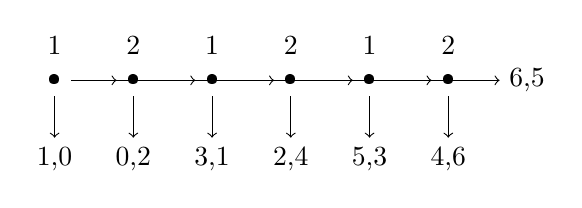
\begin{tikzpicture}
        \node [label={above: 1}] (A) at (0,0) {\textbullet};
        \node (AA) at(0,-1) {1,0};
        \node[label={above: 2}] (B)at (1,0) {\textbullet};
        \node (BB)  at (1,-1) {0,2};
        \node[label={above: 1}] (C)at (2,0) {\textbullet};
        \node (CC) at (2,-1) {3,1};
        \node[label={above: 2}] (D)at (3,0) {\textbullet};
        \node (DD)at (3,-1) {2,4};
        \node[label={above: 1}] (E)at (4,0) {\textbullet};
        \node(EE) at (4,-1) {5,3};
        \node[label={above: 2}] (F)at (5,0) {\textbullet};
        \node (FF)at (5,-1) {4,6};
        \node (G)at (6,0) {6,5};
        
            \draw[->] (A)edge (B)edge (C)edge (D)edge (E)edge (F)edge (G);\draw[->](A) edge(AA);
            \draw[->](B) edge(BB);
            \draw[->](C) edge(CC);
            \draw[->](D) edge(DD);
            \draw[->](E) edge(EE);
            \draw[->](F) edge(FF);

    \end{tikzpicture}
\end{center}
    Intuitively, the sequence should continue sometime into the right. However, the SPNE actually results in (1,0)!
\end{aexample}
Or \begin{center}
    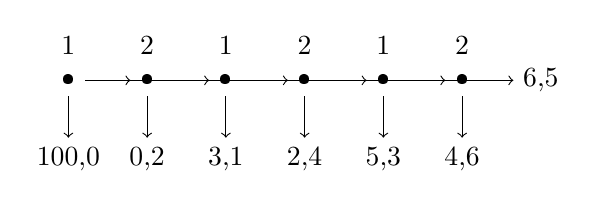
\begin{tikzpicture}
        \node [label={above: 1}] (A) at (0,0) {\textbullet};
        \node (AA) at(0,-1) {100,0};
        \node[label={above: 2}] (B)at (1,0) {\textbullet};
        \node (BB)  at (1,-1) {0,2};
        \node[label={above: 1}] (C)at (2,0) {\textbullet};
        \node (CC) at (2,-1) {3,1};
        \node[label={above: 2}] (D)at (3,0) {\textbullet};
        \node (DD)at (3,-1) {2,4};
        \node[label={above: 1}] (E)at (4,0) {\textbullet};
        \node(EE) at (4,-1) {5,3};
        \node[label={above: 2}] (F)at (5,0) {\textbullet};
        \node (FF)at (5,-1) {4,6};
        \node (G)at (6,0) {6,5};
        
            \draw[->] (A)edge (B)edge (C)edge (D)edge (E)edge (F)edge (G);\draw[->](A) edge(AA);
            \draw[->](B) edge(BB);
            \draw[->](C) edge(CC);
            \draw[->](D) edge(DD);
            \draw[->](E) edge(EE);
            \draw[->](F) edge(FF);

    \end{tikzpicture}
\end{center}
In this case, we do not even consider what player 1 would do in the right, because the first choice dominates all possiblities. It is not certain that people think of subgames.


\definition{Information set}{
    An information set is a collection of decision nodes that are indistinguishable for the player making the decision at the nodes.
}

We can also adjust the extensive form representation by drawing a circle/dashed line across indistinguishable subgames.
\begin{center}
    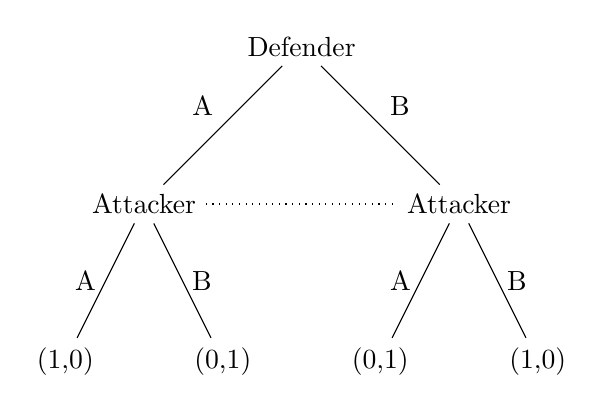
\begin{tikzpicture}
        \node (A) at (0,0){Defender};
        \node(B) at (-2,-2) {Attacker};
        \node(C) at (2,-2) {Attacker};
        \node(D) at (-3,-4) {(1,0)};
        \node(E) at (-1,-4) {(0,1)};
        \node(F) at (1,-4) {(0,1)};
        \node(G) at (3,-4) {(1,0)};
        \draw (A) edge  node[midway, above left]{A}(B);
        \draw (A) edge  node[midway, above right]{B}(C);
        \draw (B) edge  node[midway,  left]{A}(D);
        \draw (B) edge node[midway,  right]{B} (E) ;
        \draw (C) edge  node[midway,  left]{A}(F);
        \draw (C) edge  node[midway,  right]{B}(G);
        \draw [dotted] (B)edge (C);
    \end{tikzpicture}\end{center}

    In this case, the Attacker cannot distinguish the subgames depending on what the Defender picked. The defender's information set is a singleton. 
    \definition{Perfect information game}{
        If every information set is a singleton, we call the game a \textbf{game with perfect information.}
    }

\begin{aexample}{}{}
    
\begin{center}
    \begin{tikzpicture}
        \node(a) at (-2,4){1};
        \node(b) at (-3,2){(2,2)};
        \node(c) at (-1,2){2};
        \node(d) at (-2,0){(1,2)};
        \draw (a) edge  node[midway, above left]{L}(b);\draw (a) edge  node[midway, above right]{R}(c);
        \draw (c) edge node[midway, above left]{L} (d);
        \draw (c) edge node[midway, above right]{R} (A);

        \node (A) at (0,0){1};
        \node(B) at (-2,-2) {2};
        \node(C) at (2,-2) {2};
        \node(D) at (-3,-4) {(2,5)};
        \node(E) at (-1,-4) {(0,0)};
        \node(F) at (1,-4) {(3,0)};
        \node(G) at (3,-4) {(1,1)};
        \draw (A) edge  node[midway, above left]{A}(B);
        \draw (A) edge  node[midway, above right]{B}(C);
        \draw (B) edge  node[midway,  left]{C}(D);
        \draw (B) edge node[midway,  right]{D} (E) ;
        \draw (C) edge  node[midway,  left]{C}(F);
        \draw (C) edge  node[midway,  right]{D}(G);
        \draw [dotted] (B)edge (C);
    \end{tikzpicture}\end{center}
\end{aexample}
We need to work on \textbf{proper subgames}, games that start at a singleton and does not break any information set. 
Starting with the second decision tree of 1, 
payoff matrix of \begin{center}
    \begin{tabular}{|c c|}
            \hline (2,5) & (0,0)\\ \hline (3,0) & (1,1)\\ \hline
    \end{tabular}
\end{center}
has a Nash equilibrium of (B,D). Then 2 chooses between (1,2) and (1,1), so would decide L in the tree. Finally 1's first decision between (2,2) and (1,2) will lead to a SPNE result of (2,2).

\begin{aexample}{Bank Runs}{}
    There are two investors. Each puts $D$ dollars in the bank. This money is invested in a long term project.
    
    \begin{itemize}
        \item Period 1: The investors can withdraw or stay invested. Pulling out now will get a return of $2r$, $r\in (D,D/2)$.
        \item Period 2: If investment matures, the return is $2R$, $R>D$.
    \end{itemize}
    \begin{center}
    \begin{tabular}{|c|c c|}
        \hline period 1& W & S\\
            \hline  W & (r,r) & (D,2r-D)\\ \hline S& (2r-D,D) & next stage\\ \hline
    \end{tabular}
\end{center}
\begin{center}
    \begin{tabular}{|c|c c|}
        \hline period 2 & W & S\\
            \hline  W & (R,R) & (D,2R-D)\\ \hline S& (2R-D,D) & (R,R)\\ \hline
    \end{tabular}
\end{center}
\end{aexample}
Putting (R,R) into the next stage, there are two nash equilibria (r,r) and (R,R).

\begin{aexample}{Investment and Price Competition}{}
    2 Firms first decide to invest and enter a new market at a cost of $c_i$. If both enter, they compete on price (Betrand competition). If one enters, they get to be a monopolist. If no one enters, the payoffs are zero.
\end{aexample}

   
\begin{center}
    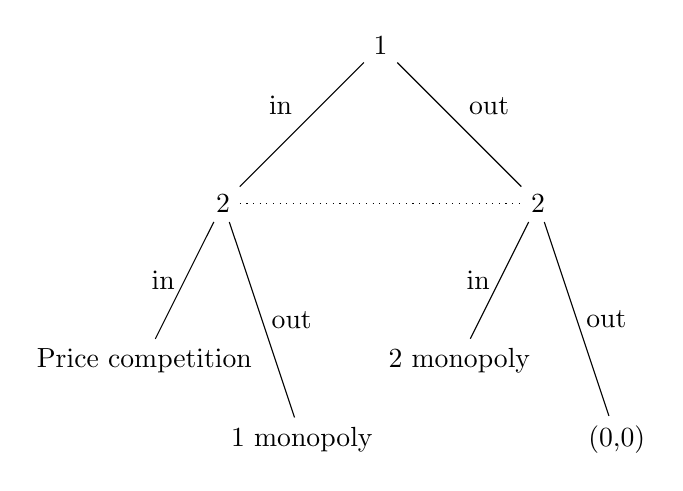
\begin{tikzpicture}
        \node (A) at (0,0){1};
        \node(B) at (-2,-2) {2};
        \node(C) at (2,-2) {2};
        \node(D) at (-3,-4) {Price competition};
        \node(E) at (-1,-5) {1 monopoly};
        \node(F) at (1,-4) {2 monopoly};
        \node(G) at (3,-5) {(0,0)};
        \draw (A) edge  node[midway, above left]{in}(B);
        \draw (A) edge  node[midway, above right]{out}(C);
        \draw (B) edge  node[midway,  left]{in}(D);
        \draw (B) edge node[midway,  right]{out} (E) ;
        \draw (C) edge  node[midway,  left]{in}(F);
        \draw (C) edge  node[midway,  right]{out}(G);
        \draw [dotted] (B)edge (C);
    \end{tikzpicture}\end{center}
    The price competition results in a payoff of $(-c_1,-c_2)$. The monopolist gains $(1/4-c_i)$.
    We therefore have a payoff matrix in the first round:
    \begin{center}
        \begin{tabular}{|c|c c|}
            \hline period 1& in & out\\
                \hline  in & $(-c_1,-c_2)$ & $(1/4-c_1,0)$\\ \hline out& $(0,1/4-c_2)$ & $(0,0)$\\ \hline
        \end{tabular}
    \end{center}
    If both $c_1,c_2>1/4$, then both will want to withdraw the market. If both of them are smaller, the nash equilibrium is that one of the firms enter the market as a Nash equilibrium. If exactly one of them has $c_i\leq 1/4$, then that firm enters the market.

    
\end{document}